\documentclass[10pt]{extarticle}
\title{}
\author{Avinash Iyer}
\date{}
\usepackage[shortlabels]{enumitem}

%font setup
\usepackage{cmbright}
%\usepackage{newpxtext,eulerpx}

%paper setup
\usepackage{geometry}
\geometry{letterpaper, portrait, margin=1in}
\usepackage{fancyhdr}

%symbols
\usepackage{amsmath}
\usepackage{amsfonts}
\usepackage{mathtools}
\usepackage[hidelinks]{hyperref}
\usepackage{gensymb}

\usepackage[T1]{fontenc}
\usepackage[utf8]{inputenc}

\usepackage[version=4]{mhchem}
\usepackage{chemfig}

%plotting
\usepackage{pgfplots}
\usepackage{tikz}
\tikzset{middleweight/.style={pos = 0.5, fill=white}}
\tikzset{weight/.style={pos = 0.5, fill = white}}
\tikzset{lateweight/.style={pos = 0.75, fill = white}}
\tikzset{earlyweight/.style={pos = 0.25, fill=white}}

%\usepackage{natbib}

%graphics stuff
\usepackage{graphicx}
\graphicspath{ {./images/} }

%code stuff
%when using minted, make sure to add the -shell-escape flag
%you can use lstlisting if you don't want to use minted
%\usepackage{minted}
%\usemintedstyle{pastie}
%\newminted[javacode]{java}{frame=lines,framesep=2mm,linenos=true,fontsize=\footnotesize,tabsize=3,autogobble,}
%\newminted[cppcode]{cpp}{frame=lines,framesep=2mm,linenos=true,fontsize=\footnotesize,tabsize=3,autogobble,}

\usepackage{listings}
\usepackage{color}
\definecolor{dkgreen}{rgb}{0,0.6,0}
\definecolor{gray}{rgb}{0.5,0.5,0.5}
\definecolor{mauve}{rgb}{0.58,0,0.82}

\lstset{frame=tb,
	language=Java,
	aboveskip=3mm,
	belowskip=3mm,
	showstringspaces=false,
	columns=flexible,
	basicstyle={\small\ttfamily},
	numbers=none,
	numberstyle=\tiny\color{gray},
	keywordstyle=\color{blue},
	commentstyle=\color{dkgreen},
	stringstyle=\color{mauve},
	breaklines=true,
	breakatwhitespace=true,
	tabsize=3
}
% text + color boxes
\usepackage[most]{tcolorbox}
\tcbuselibrary{breakable}
\tcbuselibrary{skins}
\newtcolorbox{problem}[1]{colback=white,enhanced,title={\small #1},
          attach boxed title to top center=
{yshift=-\tcboxedtitleheight/2},
boxed title style={size=small,colback=black!60!white}, sharp corners, breakable}
%including PDFs
\usepackage{pdfpages}
\setlength{\parindent}{0pt}

\pagestyle{fancy}
\fancyhf{}
\rhead{Avinash Iyer}
\lhead{Econ 308: Class Notes}
\begin{document}
  \section*{Motivations for Public Economics}%
  
  \begin{problem}{Introduction to Public Economics}
    Governments play a crucial role in much economic life.
    \begin{itemize}
      \item Regulatory structure (financial markets, pharmaceuticals, labor markets, civil rights).
      \item Taxes.
      \item Public goods and social welfare spending.
      \item Macroeconomic stabilization.
    \end{itemize}
   Public finance is the study of the role of government in a market economy, primarily focusing on taxes and spending.\\

   Reasons to study public economics:
    \begin{itemize}
      \item Governments have a lot of power in the realm of economic welfare.
      \item Nearly every economic transition is mediated by the government.
      \item It can inform debates about the appropriate role of government regarding taxes, healthcare, climate change, etc.
      \item The government is large.
        \begin{itemize}
          \item It employs 1/6 of the US Workforce.
          \item Tax revenue is approximately 27\% of the United States's Gross Domestic Product.
        \end{itemize}
    \end{itemize}
    The government (as measured by tax revenue/GDP) greatly increased in size between 1910 and 1940 (due to the establishment of the welfare state and various wars).
    \begin{center}
      \begin{tikzpicture}
            \begin{axis}[
                title = {Federal Spending (red) and Tax Receipts (blue) as a proportion of GDP},
                xlabel = {Year},
                ylabel = {Percentage of GDP},
               y tick label style={/pgf/number format/.cd,%
            scaled y ticks = false,
            set thousands separator={},
            fixed}, xmin = 1929, xmax = 2022,
                x tick label style={/pgf/number format/.cd,%
            scaled y ticks = false,
            set thousands separator={},
            fixed},ymin = 0, ymax = 45,
                ytick = {0,5,10,15,20,25,30,35,40,45},
              width=\textwidth,
              axis lines = left,height=\axisdefaultheight
              ]
               \addplot[color=blue] table[x index=0, y index=1]{receipts_expenditures.tsv};
               \addplot[color=red] table[x index=0, y index=2]{receipts_expenditures.tsv};
            \end{axis}
    \end{tikzpicture}
    \end{center}
    \begin{problem}{Two Motivations for Government Intervention}
      \begin{itemize}
        \item Market Failure
        \item Redistribution
      \end{itemize}
      The First Welfare Theorem states that \textit{in the absence of market failure}, markets will yield a result along the \textbf{utility possibilities frontier} (i.e., the set of all maximized utilities given the current market).

      However, there are a lot of market failures:
      \begin{itemize}
        \item Externalities (pollution, network effects from vaccination)
        \item Public Goods (public safety)
        \item Asymmetric Information (market for lemons)
        \item Individual Mistakes (failure to save)
        \item Imperfect Competition (oligopoly, cartelization)
      \end{itemize}
      Policymakers also have to consider the \textit{equity-efficiency tradeoff} in redistribution (i.e., some redistributive acts might reduce total utility)
    \end{problem}
    \begin{problem}{Government as Social Cooperation}
      \begin{itemize}
        \item Economists tend to have a narrow view of human behavior, but social cooperation undergirds much of the levels of societal coordination beyond individuals (i.e., families, communities, countries, global superstructures)
        \item Human societies of old depended on social cooperation for protection and taking care of the young, sick, and old.
        \item Modern states are the primary form of coordination today.
        \item Humans reveal their social nature (or social solidarity) via the size of the government (informal and formal).
      \end{itemize}
    \end{problem}
  \end{problem}
  \begin{problem}{Introduction Activity}
    \begin{tcbraster}[raster columns = 1,colframe = black!75!white,colback=white]
      \tcbincludepdf{images/Activity_1.pdf}
    \end{tcbraster}
  \end{problem}
  \begin{problem}{Microeconomic Foundations: Consumer Theory}
    \begin{description}
      \item[Utility function] $u(X,Y)$ translates consumption quantities into utility.
      \item[Indifference curve] A graphical representation of all bundles of goods that make an individual equally well off. Mathematically, an indifference curve is the set of all bundles $(X,Y)$ such that $u(X,Y) = U$ for some utility level $U$.
      \item[Marginal Rate of Substitution] $MRS_{XY}$ is the negative slope of the indifference curve --- it's the rate at which the consumer will trade $Y$ for $X$.
        \[
          MRS_{XY} = \frac{\partial u/\partial X}{\partial u/\partial Y}
        \] 
      \item[Budget Constraint] the set of all bundles for which the total amount spent equals income
        \begin{itemize}
          \item Let $I$ indicate income and $P_X$ and $P_Y$ represent the prices of goods $X$ and $Y$ respectively.
          \item The budget constraint is the line segment $P_X X + P_Y Y = I$.
          \item The slope of the budget constraint is $-\frac{P_X}{P_Y}$.
        \end{itemize}
      \item[Utility Maximization] A rational consumer maximizes utility subject to the budget constraint via the parallel conditions of tangency ($MRS_{XY} = \frac{P_X}{P_Y}$) and the budget constraint ($P_X X + P_Y Y = I$).
      \item[Demand Functions] Utility maximization generates demand functions (quantity in terms of price) $X(P_X,P_Y,I)$ and $Y(P_X,P_Y,I)$. There are two primary canonical utility functions.
        \begin{itemize}
          \item Cobb-Douglas: $u(X,Y) = A\ln(X) + B\ln(Y)$, or $u(X,Y) = X^A \cdot Y^B$. The demand function for this utility function yields that $P_X$ has no effect on $Y$ and $P_Y$ has no effect on $X$.
          \item Quasilinear: $u(X,Y) = v(X) + BY$ where $v'(X)>0>v''(X)$ (i.e., concave down, sloping up). The demand function for this utility function yields that $I$ has no effect on $X$ assuming an interior solution.
        \end{itemize}
      \item[Price Effects] The impact of a change in $P_X$ on demand for $X$ is composed into two effects:
        \begin{itemize}
          \item Substitution Effect: change in consumption due to the change in relative prices, with utility held equal. When the price of a good increases, the substitution effect is always negative, and vice versa.
          \item Income Effect: change in consumption due to a change in purchasing power as a result of the price change, where relative prices are held constant at the final price ratio. Income effects can be positive or negative depending on the type of good.
          \item The total effect is equal to the income effect and the substitution effect.
        \end{itemize}
    \end{description}
    \begin{center}
      \begin{tcbraster}[raster columns = 1,colframe = black!75!white,colback=white,title=Income and Substitution Effects]
        \tcbincludepdf[width=10cm]{images/income_substitution.pdf}
      \end{tcbraster}
    \end{center}
    \begin{description}
      \item[Price Elasticity] The price elasticity of demand is the \% change in demand caused by a 1\% change in price of a good.
        \[
          E^D = \frac{dD}{dP}\frac{P}{D}
        \] 
      Elasticities are \textit{unit-free}, typically negative, and tend not to be constant along a demand curve.
    \end{description}
  \end{problem}
  \begin{problem}{Game Theory}
    Some decision problems involve strategic interactions between individuals.
    \begin{itemize}
      \item For example, Antonia and Bruno might care about giving to a local charity, and give $G_A$ and $G_B$ respectively. 
      \item Their utility functions depend on each other $u_A(G_A,G_B),u_B(G_A,G_B)$.
      \item The \textbf{Nash Equilibrium} yields each individual choosing an action that maximizes their utility \textit{given the other person's behavior}.
    \end{itemize}
  \end{problem}
  \begin{problem}{Social Welfare}
    Economists incorporate distributional concerns by use of social welfare functions.
    \[
      SWF = f(U_1,U_2,\dots,U_n)
    \] 
    We have two canonical social welfare functions:
    \begin{itemize}
      \item Utilitarian SWF: $SWF = U_1 + U_2 + \cdots U_n$.
      \begin{itemize}
        \item Marginal utility decreasing in income $\rightarrow$ redistribution from the rich to the poor.
        \item Taking \$1 from a rich person decreases their utility by a small amount, but transferring to a poor person increases their utility by a large amount.
      \end{itemize}
      \item Rawlsian SWF: $SWF = \min\{U_1,U_2,\dots,U_N\}$
      \begin{itemize}
        \item Social welfare is maximized by maximizing the well-being of the worst-off person.
        \item Rawlsian social welfare is more redistributive than utilitarian social welfare.
      \end{itemize}
    \end{itemize}
    There are a few other philosophies regarding the fairness of economic distribution in society.
    \begin{description}
      \item[Just deserts] Individuals should be compensated in line with their contributions.
      \item[Commodity egalitarianism] Society should ensure that individuals meet a set of basic needs, but beyond that point income distribution is irrelevant.
      \item[Equality of opportunity] Society should ensure that all individuals have equal opportunities for success.
    \end{description}
  \end{problem}
  \begin{problem}{Present Discounted Value}
    The present discounted value of a future value of money $F$ that is received and spent in $n$ periods is:
    \[
      PDV = \frac{F}{(1+r)^n}
    \] 
    For the \textbf{discount rate} $r$, typically the interest rate.\\

    For a stream of future expenses $F_i$, we use the following formula:
    \[
      PDV = \sum_{i = 1}^{n} \frac{F_i}{(1+r)^i}
    \] 
    If the values of $F_i$ are equal, then $PDV = \frac{F}{r}$, via the geometric series formula.
  \end{problem}
  \begin{problem}{Theoretical Tools Activity}
   \begin{tcbraster}[raster columns = 1,colframe = black!75!white,colback=white]
     \tcbincludepdf{images/Activity_2.pdf}
   \end{tcbraster} 
  \end{problem}
  \begin{problem}{Empirical Tools of Public Economics}
    \textbf{Identification Problem}: When two variables, $A$ and $B$, are correlated with each other, how do you identify which is causing which (or if both are being caused by something else)? Could the correlation be spurious?
    \begin{problem}{Spurious Correlation}
      \begin{tcbraster}[raster columns = 1,colframe = black!75!white,colback=white]
        \tcbincludepdf{images/spurious_correlation.pdf}
      \end{tcbraster}
    \end{problem}
    \begin{problem}{Randomized Controlled Trials}
      The gold standard of experimentation.
      \begin{itemize}
        \item One group obtains the treatment, one gets the placebo.
        \item The two groups must have close to identical traits aside from the treatment, which is part of the ``control.''
      \end{itemize}
      Randomized controlled trails tend to be common in science, and have grown in popularity in the social sciences, but for economics, RCTs are often difficult to carry out (after all, you cannot split up the timeline).
      \begin{problem}{Limitations of RCTs}
        External validity: it's difficult to apply the outcomes of a randomized controlled trial to other contexts.\\

        Attrition: unequal loss of participants (i.e., people in the control group drop out more than the treatment group, or vice versa).\\

        Unethicality: little feedback on the part of participants, and the interests of participants aren't necessarily taken into account.
      \end{problem}
    \end{problem}
    \begin{problem}{Observational Data}
      Data generated by individual behavior observed in the real world, not in specially-designed experiments.
      \begin{itemize}
        \item Time Series analysis: changes in two different stats over time and trying to find results from said changes.
        \item Cross-Sectional Regression Analysis: finding a relationship between two variables with many data samples.
          \[
            Y_i = \alpha + \beta X_i + \epsilon_i
          \] 
          The OLS estimate, $\hat{\beta}$, is the slope of the data. In order for this relationship to be causal, the error term, $\epsilon_i$, must be uncorrelated with $X_i$.
      \end{itemize}
    \end{problem}
    \begin{problem}{Quasi-Experiments}
      Changes in the economic environments that create nearly identical treatment and control groups for studying the effect of that environmental change, allowing economists to take advantage of quasi-randomization created by external forces.
    \end{problem}
  \end{problem}
  \begin{problem}{Empirical Tools Activity}
   \begin{tcbraster}[raster columns = 1,colframe = black!75!white,colback=white]
     \tcbincludepdf{images/Activity_3.pdf}
   \end{tcbraster}
  \end{problem}
  \section*{Market Failures}%
  \begin{problem}{Market Failures: Externalities}
    The most classic market failure is \textit{externalities}: when the fully private costs/benefits and the social costs/benefit are misaligned. For example, possibly the most important example of a \textit{negative} externality is climate change from CO$_2$ emissions, a byproduct of industrial development.\\

    Economists focus on balancing the total costs (private + social) of pollution with the total benefits (private + social) from pollution.
    \begin{center}
      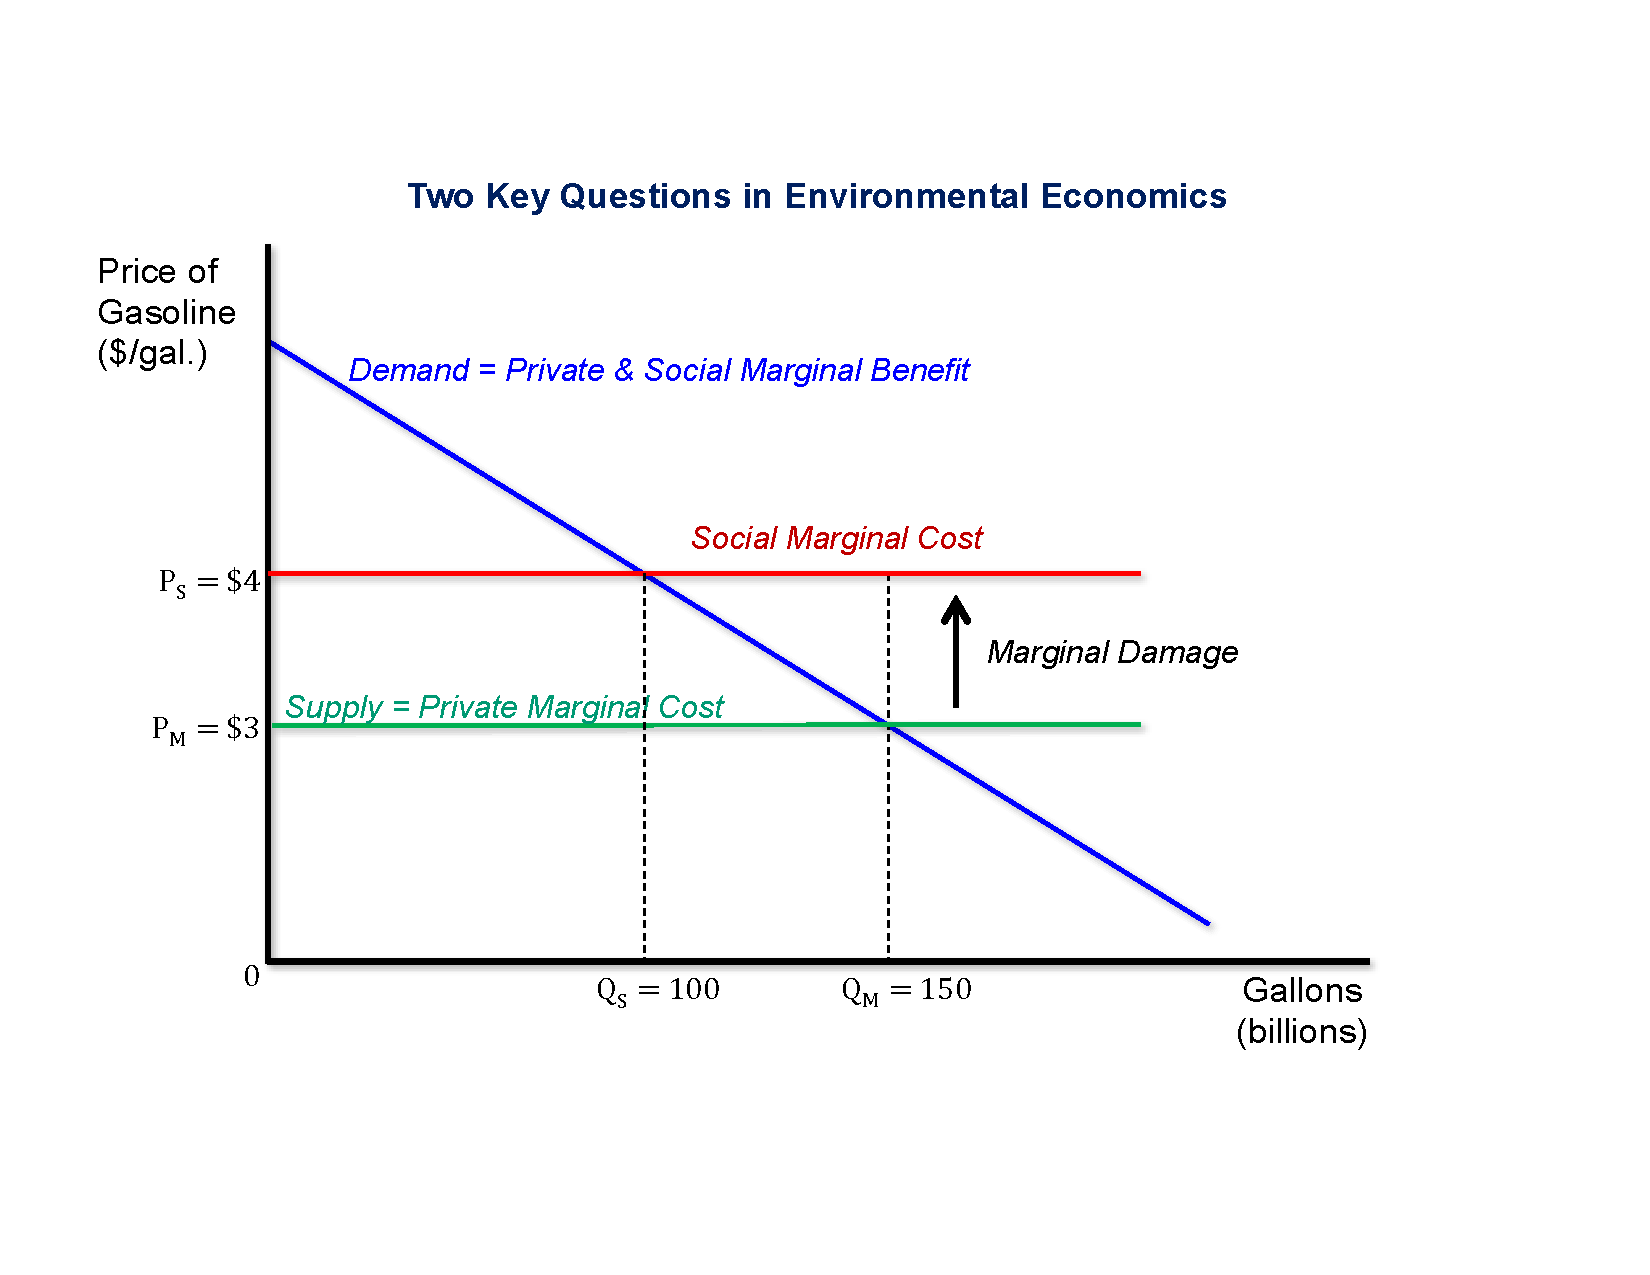
\includegraphics[width=\textwidth]{climate_change_externalities.pdf}
    \end{center}
    The top triangle represents the deadweight loss because the problem of underpriced externalities is one of \textit{overproduction}, not of underproduction. We are facing two questions:
    \begin{itemize}
      \item How do we calculate the marginal social cost of pollution?
      \item What is the best way to reach the marginal social cost of pollution?
    \end{itemize}
    \begin{problem}{Estimating the social cost of carbon}
      \begin{description}
        \item[Step 1:] How does one extra ton of CO$_2$ impact the climate?
        \item[Step 2:] How does a marginal change in climate affect various human outcomes?
        \item[Step 3:] Calculate the current social cost by converting future costs into current dollars via discounting.
      \end{description}
      For Step 2, economists control for the particular location, and do comparisons over time, and check the average effect across all the locations.\\

      After calculating or estimating future costs, economists need to discount these costs toward the present value.
      \[
        PDV = \frac{C_1}{1+r} + \frac{C_2}{(1+r)^2} + \cdots
      \] 
      where $r$ is the \textit{social discount rate}, the rate at which society is willing to trade off between consumption today and consumption tomorrow.\\

      Changes in $r$ matter a lot:
      \begin{itemize}
        \item If $r$ is large (i.e., we don't care much about future generations), then carbon costs are not large.
        \item If $r = 0$ (i.e., we care equally about all generations), then carbon costs can be infinite.
      \end{itemize}
      Various economists calculated different social discount rates:
      \begin{itemize}
        \item Giglio, Maggiori, and Stroebel calculated $2.6\%$, by using differences in price between perpetual ownership and 100 year leases.
        \item The Obama administration used a 3\% discount rate, implying the social cost of carbon was \$42/ton.
        \item The Trump administration used a 7\% discount rate, implying the social cost of carbon was \$5/ton
        \item The Biden administration uses an estimate of \$51/ton.
      \end{itemize}
    \end{problem}
  \end{problem}
  \begin{problem}{Policy Solutions}
    We can use \textit{pigouvian taxes} to force market participants to internalize the cost of the externality.\\

    Alternatively, we can use \textit{industrial policy}, to restructure the market in order to pursue a public goal.
    \begin{itemize}
      \item Subsidizing clean energy.
      \item Research in clean energy technologies both public and private.
      \item Phase out carbon in various economic sectors and weaken fossil fuels.
    \end{itemize}
    We have seen great dividends so far: solar and wind have become extremely cheap to produce, and replacing coal with natural gas has yielded emissions reductions that were greater than targets. The Biden administration focused on making clean energy even cheaper via the Inflation Reduction Act.
  \end{problem}
  \begin{problem}{Externalities Activity}
    \begin{tcbraster}[raster columns = 1,colframe = black!75!white,colback=white]
      \tcbincludepdf{images/Activity_4.pdf}
    \end{tcbraster}
  \end{problem}
  \begin{problem}{Public Goods}
    A public good is not something that's merely good for the public, but it is specifically a good that is rival and non-excludable (essentially, the same quantity of the good has to be available to every person.)\\

    The optimal level of publi goods is when the \textit{vertical} sum of individual demand curves equals the marginal cost of providing the public good. The reason the demand curves are added vertically is because market participants can share the public goods.\\

    Recall that $MRS_{GX}$ of a public good $G$ for a private good $X$ is how much an individual values an additional unit of $G$ in terms of unit of $X$.
    \begin{align*}
      MRS_{GX} &= \frac{MU_G}{MU_X}
    \end{align*}
    The total number of units of $X$ society is willing to give up for $1$ more unit of $G$ is the sum of all $MRS_{GX}$.\\

    Assuming that $P_X = 1$, this is a measure of how many dollars society is willing to pay for $1$ more unit of $G$. The societal value is the sum of the different $MRS_{GX}$ values:
    \begin{align*}
      MC_G &= \sum_{I=1}^{N} MRS_{GX}^I
    \end{align*}
    This is the \textit{Samuelson Rule}.
  \end{problem}
  \begin{problem}{Private Provision of Public Goods}
    \begin{itemize}
      \item The private outcome is the Nash equilibrium of a game where individuals choose how to allocate income between $G$ and $X$, taking into account spending on $G$ by others.
      \item The Nash equilibrium does not satisfy the Samuelson Rule.
      \item Public goods problems can be described as \textbf{free-rider} problems (i.e., underproduction).
      \item There is not necessarily zero private provision of public goods. Private provision works well in the following cases:
        \begin{itemize}
          \item Some people have much higher marginal rate of substitution (i.e., they care more than others).
          \item Altruism: people care purely about giving to others.
          \item Warm Glow: people get utility from giving to others.
        \end{itemize}
    \end{itemize}
    There is experimental evidence of free-riding; for example, Marwell and Ames (1981) had an experiment where they tested whether subjects were willing to contribute to a public good, where the Nash equilibrium was that people didn't contribute, and the social optimum was everyone contributing.\\

    People are willing to cooperate at first, but then get upset as time goes on and retaliate.
  \end{problem}
  \begin{problem}{Public Goods Example}
    Let there be $2$ people, with the same utility functions over $X,F$, where $X$ is a private good and $F$ is a public good:
    \begin{align*}
      U_i(X_i,F) &= 2\ln(X_i) + \ln(F)\tag*{for $i=1,2$}
    \end{align*}
    Each participant has a budget constraint, where $P_X$ and $P_F$ are both $1$.
    \begin{align*}
      X_i + F_i = 100\tag*{for $i=1,2$}
    \end{align*}
    Where $F = F_1 + F_2$.
    \begin{description}
      \item[Maximize Person 1's utility:] (i.e., finding the best response function)
    \end{description}
    \begin{align*}
      0 &= \frac{\partial U_1}{\partial F_1}\\
      0 &= -\frac{2}{100-F_1} + \frac{1}{F_1 + F_2}\tag*{recall that $X_1 = 100-F_1$}\\
      2(F_1 + F_2) &= 100-F_1\\
      F_1 &= \frac{100-2F_2}{3}
    \end{align*}
    Since this is a symmetric game, we know that the best response function for Person 2 is $F_2 = \frac{100-2F_1}{3}$.\\

    The Nash equilibrium is when all players are playing their best response to each other. Since the game is symmetric, we know that $F_1^* = F_2^*$
    \begin{align*}
      F_1^* &= \frac{100-2F_1^*}{3}\\
      F_1^* &= 20\\
      F_2^* &= 20
    \end{align*}
    The social optimum (following the Samuelson Rule) is as follows:
    \begin{align*}
      MRS_{FX}^1 + MRS_{FX}^2 &= 1\\
      \frac{MU_F}{MU_{X_1}} + \frac{MU_F}{MU_{X_2}}  &= 1\\
      \frac{1}{2}\frac{X_1}{F} + \frac{1}{2}\frac{X_2}{F} &= 1\\
      2 &= \frac{X_1 + X_2}{F}\\
      F &= \frac{X_1 + X_2}{2}\\
      F &= \frac{200-F}{2}\\
      F &= \frac{200}{3}
    \end{align*}
  \end{problem}
  \begin{problem}{Public Provision of Public Goods}
    The primary problem of public provision of public goods is \textit{crowding out} (i.e., reduced private contributions to public goods). There are two key assumptions of one-to-one private contributions:
    \begin{itemize}
      \item Individuals do \textit{not} have warm glow preferences.
      \item Private actors are contributing to the public good.
    \end{itemize}
    There is empirical evidence of partial crowd-out (i.e., reduction in charitable giving as government spending is increased). However, since people tend to give to charity due to warm glow preferences and social pressures, the crowd-out is not one-to-one. Hungerman (2005) estimates that the crowd-out effect is 20–40 cents per dollar of welfare spending.
  \end{problem}
  \begin{problem}{Public Goods Activity}
    \begin{tcbraster}[raster columns = 1,colframe = black!75!white,colback=white]
      \tcbincludepdf{images/activity_5.pdf}
    \end{tcbraster}
  \end{problem}
  \begin{problem}{Three Questions in Public Economics}
    \begin{description}
      \item[Descriptive:] What are the effects of interventions and policies (empirical)?
      \item[Normative:] What is the optimal policy (theoretical)?
      \item[Public Choice:] Why do governments choose the policies they do (mixture of theory and empirics)?
    \end{description}
  \end{problem}
  \begin{problem}{Rules of Social Decision}
    There are at least 2 individuals with transitive preferences over at least $3$ options. A \textbf{social decision rule} aggregates these preferences into a social preference over these options.\\

    Suppose we want our social decision rule to satisfy the following properties:
    \begin{description}
      \item[Transitive:] if $a$ is ranked above $b$ by our rule, and $b$ is ranked above $c$ by our rule, then $a$ has to be ranked above $c$ by our rule.
      \item[Pareto Efficiency:] if everyone prefers $a$ to $b$, then our rule should rank $a$ above $b$.
      \item[Independence of Irrelevant Alternatives:] the ranking of any two options depends only on how individuals rank the options (and not the ranking of other alternatives).
      \item[Non-dictatorship:] There is no individual whose preference ranking of any two options matches the social ranking (no matter the preferences of others).
    \end{description}
    All of these seem reasonable, so they must be possible, right? Well...
  \end{problem}
  \begin{problem}{Arrow's Impossibility Theorem}
    Arrow's Impossibility Theorem is the following:
    \begin{quote}
        There is no social decision rule that satisfies the properties of Universality (i.e., transitivity), Pareto Efficiency, Independence of Irrelevant Alternatives, and Non-dictatorship.
    \end{quote}
    The implication of Arrow's Impossibility Theorem means that the only voting method that satisfies the first three properties of our social rule is a dictatorship. However, since we don't want a dictatorship, we can use the following:
    \begin{itemize}
      \item Restrict preferences (i.e., transitive is insufficient)
      \item Relax Independence of Irrelevant Alternatives, and let intensity of preferences play a role (for example, the Samuelson rule).
    \end{itemize}
  \end{problem}
  \begin{problem}{Case Study: Majority Voting}
    Pairwise majority voting is a mechanism to aggregate individual votes into a social decision. Since Majority Voting is obviously Pareto efficient and non-dictatorial, and satisfies IIA because the ranking of $a$ over $b$ only depends on how many people vote $a$ vs. how many people vote $b$. Therefore, we must have that majority voting fails transitivity.\\

    Consider an election for funding public schools:
    \begin{problem}{Majority Voting ``Working''}
      \begin{center}
        \renewcommand{\arraystretch}{1.5}
        \begin{tabular}{c|c|c|c|}
          \multicolumn{1}{c}{Preferences} & \multicolumn{3}{c}{Type of Voter}\\
          \cline{2-4}
                                          & Parents ($1/3$) & Elders ($1/3$) & Young Couples ($1/3$)\\
          \cline{2-4}
          First & $H$ & $L$ & $M$\\
          \cline{2-4}
          Second & $M$ & $M$ & $L$\\
          \cline{2-4}
          Third & $L$ & $H$ & $H$\\
          \cline{2-4}
        \end{tabular}
      \end{center}
      \begin{itemize}
        \item $M>_s L$
        \item $L >_s H$
        \item $M >_s H$
      \end{itemize}
      Therefore, $M>L>H$, and so $M$ is the social choice made by pairwise majority voting.
    \end{problem}
    \begin{problem}{Majority Voting ``Failing''}
      \begin{center}
        \renewcommand{\arraystretch}{1.5}
        \begin{tabular}{c|c|c|c|}
          \multicolumn{1}{c}{Preferences} & \multicolumn{3}{c}{Type of Voter}\\
          \cline{2-4}
                                          & Public School ($1/3$) & Private School ($1/3$) & Young Couples ($1/3$)\\
          \cline{2-4}
          First & $H$ & $L$ & $M$\\
          \cline{2-4}
          Second & $M$ & $H$ & $L$\\
          \cline{2-4}
          Third & $L$ & $M$ & $H$\\
          \cline{2-4}
        \end{tabular}
      \end{center}
      \begin{itemize}
        \item $M >_s L$
        \item $L >_s H$
        \item $H >_s M$
      \end{itemize}
      We are now stuck in a cycle $M>L>H>M>\cdots$. This election fails to successfully aggregate the preferences of the populace.
    \end{problem}
    A way to get out of the trap of transitivity is to rule out preferences that are not single-peaked (i.e., one local maximum).\\

    However, when we have single-peaked preferences, we have that the preferences of the median voter is that which is preferred by society.
  \end{problem}
  \begin{problem}{Implications of the Median Voter Theorem}
    If we restrict our analysis to single-peaked preferences, majority voting is a social decision rule that satisfies all desirable properties.\\

    However, this means majority voting does not imply efficiency. For example, if a public good is efficient, but because a minority has a large marginal benefit and the majority has a small marginal benefit, the public good will get rejected. What matters for efficiency is the \textit{average} marginal benefit across individuals, not the \textit{median} marginal benefit.\\

    However, the median voter theorem doesn't really hold in real life (i.e., Democrats close to the median still vote similar to their caucus, and Republicans close to the median still vote similar to their caucus).
  \end{problem}
  \begin{problem}{Political Economy Activity}
    \begin{tcbraster}[raster columns = 1,colframe = black!75!white,colback=white]
      \tcbincludepdf{images/activity_6.pdf}
    \end{tcbraster}
  \end{problem}
  \begin{problem}{Local Public Goods: the Tiebout Hypothesis}
    Tiebout (1956) asks the following: What is it about the private market that guarantees optimal provision of private goods that is missing in the case of public goods?\\

    Proposed answer: \textbf{shopping} and \textbf{competition}. However, we can see this somewhat resolved in the local level:
    \begin{itemize}
      \item Individuals can vote with their feet (i.e., move between different cities)
      \item The threat of exit can induce competition in the provision of public goods.
    \end{itemize}
    \begin{quote}
        Just as the consumer may be visualized as walking to a private market place to buy his goods,... we place him in the position of walking to a community where the prices (taxes) of community services are set. Both trips take the consumer to the market. There is no way in which the consumer can avoid revealing his preferences in a spatial economy.
    \end{quote}
  \end{problem}
  \begin{problem}{Modeling the Tiebout Hypothesis}
    Suppose there are $2N$ families, each with identical income $Y$, and 2 towns with $N$ homes each.\\

    Towns $1$ and $2$ supply levels $G_1$ and $G_2$ of local public goods at $MC_G = 1$.
    \begin{itemize}
      \item $N$ families with kids, with $U^K(C,G)$ over private consumption $C$ and public schools $G$.
      \item $N$ elderly families, with $U^E(C)$ over only private consumption $C$.
    \end{itemize}
    The allocation of families across towns is a \textbf{Tiebout Equilibrium} if and only if:
    \begin{enumerate}[(1)]
      \item No two families want to exchange locations across towns; and
      \item In each town, $G$ is decided by the median voter and financed \textit{equally} by town residents.
    \end{enumerate}
    \begin{description}
      \item[Family Budget Constraint:] $Y = C + G/N$, where $P_C = 1$ and $P_G = 1/N$
        \begin{itemize}
          \item If the majority in the town is elderly, then $G = 0$, as that maximizes $U^E(Y-G/N)$. 
          \item If the majority in the town is families with kids, then $G^*$ is that which maximizes $U^K(Y-G/N,G)$ such that $MRS_{GC}^K = \frac{1}{N}$.
        \end{itemize}
    \end{description}
    \begin{problem}{Tiebout Theorem}
      \begin{description}
        \item[Part 1 (Sorting):] In equilibrium, families will sort themselves in towns according to their taste for the public good (1 town with elderly only, one town with families with kids).
        \item[Part 2 (Efficiency):] In each town, the level of local public good is efficient.
          \begin{itemize}
            \item In the elderly town, $G = 0$, which is efficient as nobody values $G$.
            \item In the kids town, $\sum MRS_{GC}^{K} = \frac{1}{N} = 1 = MC_G$, which is the Samuelson Rule for efficiency in public goods provision.
          \end{itemize}
      \end{description}
    \end{problem}
    A Tiebout equilibrium may not be socially desirable if there is a public interest in integration within towns and for reducing social distance across groups (i.e., intergroup contact theory).
  \end{problem}
  \begin{problem}{Assumptions of the Tiebout Hypothesis}
    \begin{enumerate}[(1)]
      \item High Mobility: may be impeded by (artificial or natural) barriers to entry, preferences over other qualities.
      \item Perfect information: lack of knowledge about the quality of public goods.
      \item Scale: inability to fund public goods for one's preferences.
      \item Variety: enough options of types of towns.
      \item No externalities or spillovers: otherwise, public good will be underproduced.
      \item Equal financing of the public good (poll tax): local public finance generally tends to be based on property or sales tax.
    \end{enumerate}
  \end{problem}
  \begin{problem}{Financing Local Public Goods}
    \begin{itemize}
      \item Towns finance their local public goods through property taxation, where the rich pay more than the poor.
      \item Property taxes induce the poor to chase the rich, while the rich want to segregate themselves from the poor.
      \item The rich tend to implement mechanisms to prevent free-riding: making houses expensive.
        \begin{itemize}
          \item Zoning laws restrict supply of housing.
        \end{itemize}
      \item Discriminatory practices (such as deed restrictions) to stop poorer people from living near rich people.
    \end{itemize}
  \end{problem}
  \begin{problem}{Tiebout Implications for Redistribution}
    It's very hard for a local government to redistribute from the rich to the poor (easy exit).\\

    In localities, to avoid migration, public goods financing needs to have strong \textbf{tax-benefit linkages} (i.e., the relationship between taxes and the government benefits need to be very explicit and visual).\\

    Higher levels of government can redistribute across communities using taxes to directly or indirectly incentivize public goods spending.\\

    For example, state governments can match, in which case the price of public goods goes from $1$ to  $\frac{1}{1+m}$, for $m$ being the value of the match. However, with any intergovernmental transfers (either matching or intergovernmental transfer), there is a potential for crowd-out.
  \end{problem}
  \begin{problem}{Flypaper Effect}
    Empirical evidence suggests that the crowd-out of state spending by federal spending is low and often close to zero --- ``the money sticks where it lands.''\\

    More recent studies show that while there is a flypaper effect in the short run, there is substantial crowd-out from block grants in the long run.
  \end{problem}
  \begin{problem}{Local Public Goods Activity}
    \begin{tcbraster}[raster columns = 1,colframe = black!75!white,colback=white]
      \tcbincludepdf{images/activity_7.pdf}
    \end{tcbraster}
  \end{problem}
  \begin{problem}{Education: Motivations for Government Intervention}
    Education is one of the largest public goods provided by the government: 6\% of GDP and 12.7\% of total government expenditure.\\

    However, education is not a pure public good:
    \begin{itemize}
      \item Excludable: private education that charges money, or only allow a particular enrollment area.
      \item Rival: there are a limited number of seats in a school (capacity constraints, quality degrades if there are too many students).
      \item Private returns: your investment in education primarily benefits you.
    \end{itemize}
    So, why should the government be involved?
    \begin{itemize}
      \item Positive Externalities: a more educated workforce might lead to more productivity and technology.
      \item Family Failures: if the parental units are unable to provide for education that the child desires, the government involvement is welfare-improving.
      \item Borrowing constraints: education can be very expensive, and loans are less available (no collateral).
      \item Behavioral Mistakes: maybe you don't know what's in your best interest.
    \end{itemize}
  \end{problem}
  \begin{problem}{Education Reform}
    \begin{description}
      \item[Supply-Side:] Improving the process of education:
        \begin{itemize}
          \item Smaller classes
          \item Improving teachers
          \item Charter Schools
        \end{itemize}
      \item[Demand-Side:] Improving individual funding:
        \begin{itemize}
          \item Vouchers
          \item Subsidies/Loans/Grants
        \end{itemize}
    \end{description}
    \begin{problem}{Class Size}
      We cannot simply compare outcomes for students in small vs. large classes because of omitted variables (like income/family education).\\

      In Sweden, class size cuts off at 30 students --- this yields quasi-experimental variation, which we can use to see causality. Frederiksson, Ockert, and Oosterbeek (2013) found that there was a 4\% jump in wages for students in a smaller class.
    \end{problem}
    \begin{problem}{Teacher Quality}
      One measure of teacher quality: teacher value-added or test score-based metrics of teacher performance.
      \begin{itemize}
        \item How much does a teacher raise their students' test scores on average (adjusting for noise and controlling for differences in students)?
      \end{itemize}
      How do we measure the impact of teacher quality?
      \begin{itemize}
        \item The ideal RCT randomizes students to teachers with different levels of value-added.
        \item Quasi-Experiment: use the turnover in teachers across school years.
      \end{itemize}
      Chetty, Friedman, and Rockoff (2014) use data on all kids who went to NYC public schools in 1989 and link to tax records.\\

      They found an increase of 1.5\% in earnings and 1.5\% reduction in teenage births going from a 5th percentile teacher to a 95th percentile teacher.\\

      Most school districts do not use any performance measures to evaluate teachers.
    \end{problem}
    \begin{problem}{Charter Schools}
      Charter schools are schools financed with public funds that are not usually under the direct supervision of local school boards or subject to state regulation.\\

      To measure effectiveness, one cannot simply compare outcomes at charters with public schools due to different types of students.\\

      Quasi-experiment: compare charter lottery winners with charter lottery losers (for schools that use a lottery).\\

      In Massachusetts, Angrist, Pathak, and Walters (2013) found that urban charter schools boost achievement while non-urban charters reduce achievement.\\

      Charters tend to constitute a market-based approach to education, but there are some limitations:
      \begin{itemize}
        \item Demand-side limitations: Families may not have enough information to choose the best charter schools for their children.
        \item Supply-side limitations: Schools have an incentive to reject less-qualified applicants (nicknamed ``cream-skimming'').
      \end{itemize}
    \end{problem}
    \begin{problem}{Vouchers}
      With free public education, there is an incentive to \textit{cluster} their total education spend around where the public school's funding is. However, if the money for public education is given equally to all families, it's akin to a conditional block grant.\\

      Vouchers are meant to induce every household to increase their spending on education.\\

      However, there are mixed results from using vouchers:
      \begin{itemize}
        \item Angrist et al. (2002), using lottery assignment of vouchers in Colombia, show positive effects on education.
        \item Abdulkadiroglu, Pathak, and Walters (2018) used randomized lotteries to evaluate the Louisiana Scholarship program, and found lower achievement by those who win vouchers compared to those who did not.
      \end{itemize}
    \end{problem}
  \end{problem}
  \begin{problem}{Government Involvement in Higher Education}
    \begin{itemize}
      \item State Provision (about \$82 billion)
      \item Pell Grants (\$22.4 billion)
      \item Direct Student Loans (\$34.4 billion)
      \item Other reliefs (\$10.3 billion)
    \end{itemize}
    Supply trends:
    \begin{itemize}
      \item Priate non-profit universities have inelastic supply (fixed student bodies).
      \item Historically, supply for higher education has been administered by public universities (creating new UCs/Cal States/etc.)
      \item Supply has been provided by for-profit schools, although for-profit schools tend to provide little in benefits to students.
    \end{itemize}
    Reduced (direct) state funding has led to higher tuition and student debt.\\

    Additionally, women have been earning many more higher education degrees than men.\\
    \begin{problem}{Effect of Higher Education on Mobility}
      Chetty et al. (2017) study parental income and student earning outcomes by college.\\

      Certain schools (Harvard and Berkeley) tend to have high quantities of students in the top 20\% of the income distribution, while others like SUNY-Stony Brook tend to have more equal student populations.\\

      They found that education tends to have a flattening effect (i.e., poor kids and rich kids tend to have more similar outcomes when educated).\\

      The mobility rate for a given school can be found by (i.e., the rate of children born in the bottom quintile ending up in the top quintile) can be calculated by finding the success rate (probability that a child moves from the bottom quintile to the top quintile) and multiplying by the proportion of parents in the bottom quintile.\\

      The top college by mobility rate was Cal State LA, and the top ten tended to be open-access public universities (i.e., Glendale Community College, City University of New York, etc.).
    \end{problem}
  \end{problem}
  \begin{problem}{Insurance Theory}
    The \textbf{expected utility model} helps study decision under uncertainty.
    \begin{align*}
      E(u(I)) &= \sum p_k u(I_k)
    \end{align*}
    A \textbf{risk-averse} individual is someone who prefers a certain given income to a risky income with the same expected value.\\

    Risk-averse individuals will \textit{demand} insurance in order to smooth their consumption across uncertain states of the world.\\

    Consider health insurance and assume the following:
    \begin{itemize}
      \item $U(c)$ is increasing and concave.
      \item The person has income $W$
      \item The person is sick with probability $q$
      \item If sick, the person incurs medical cost $d$
      \item The expected utility without insurance: $EU^{\text{No Ins}} = (1-q)U(W) + qU(W-d)$
    \end{itemize}
    \begin{center}
      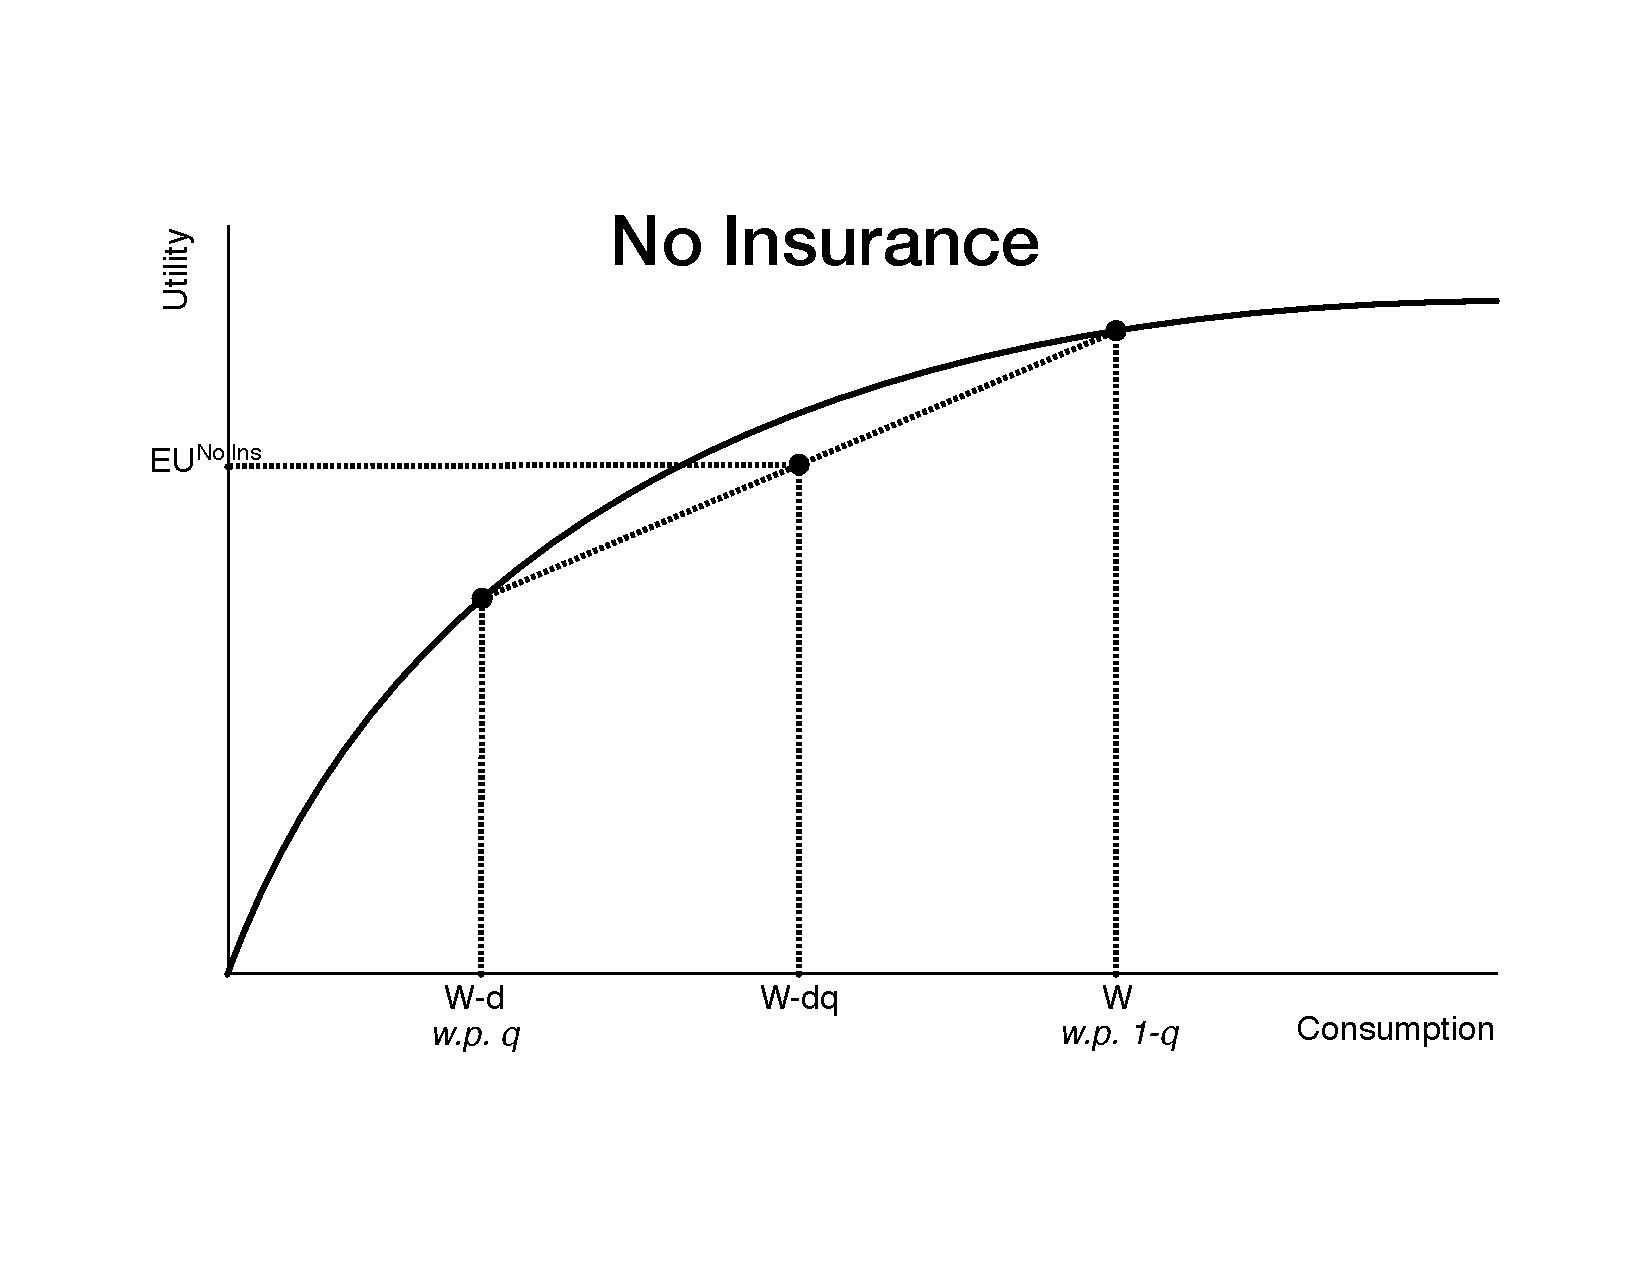
\includegraphics[width=10cm]{images/no_insurance_expected_utility.pdf}
    \end{center}
    \begin{itemize}
      \item In an insurance contract, a person pays premium $p$ always and receives $b$ only if sick.
      \item The insurance company's expected profit is $E_{\pi} = p - qb$.
      \item In perfect competition, $E_{\pi} = 0$, implying that $b = \frac{p}{q}$, which is when the insurance contract is \textbf{actuarially fair}.
    \end{itemize}
    \begin{center}
      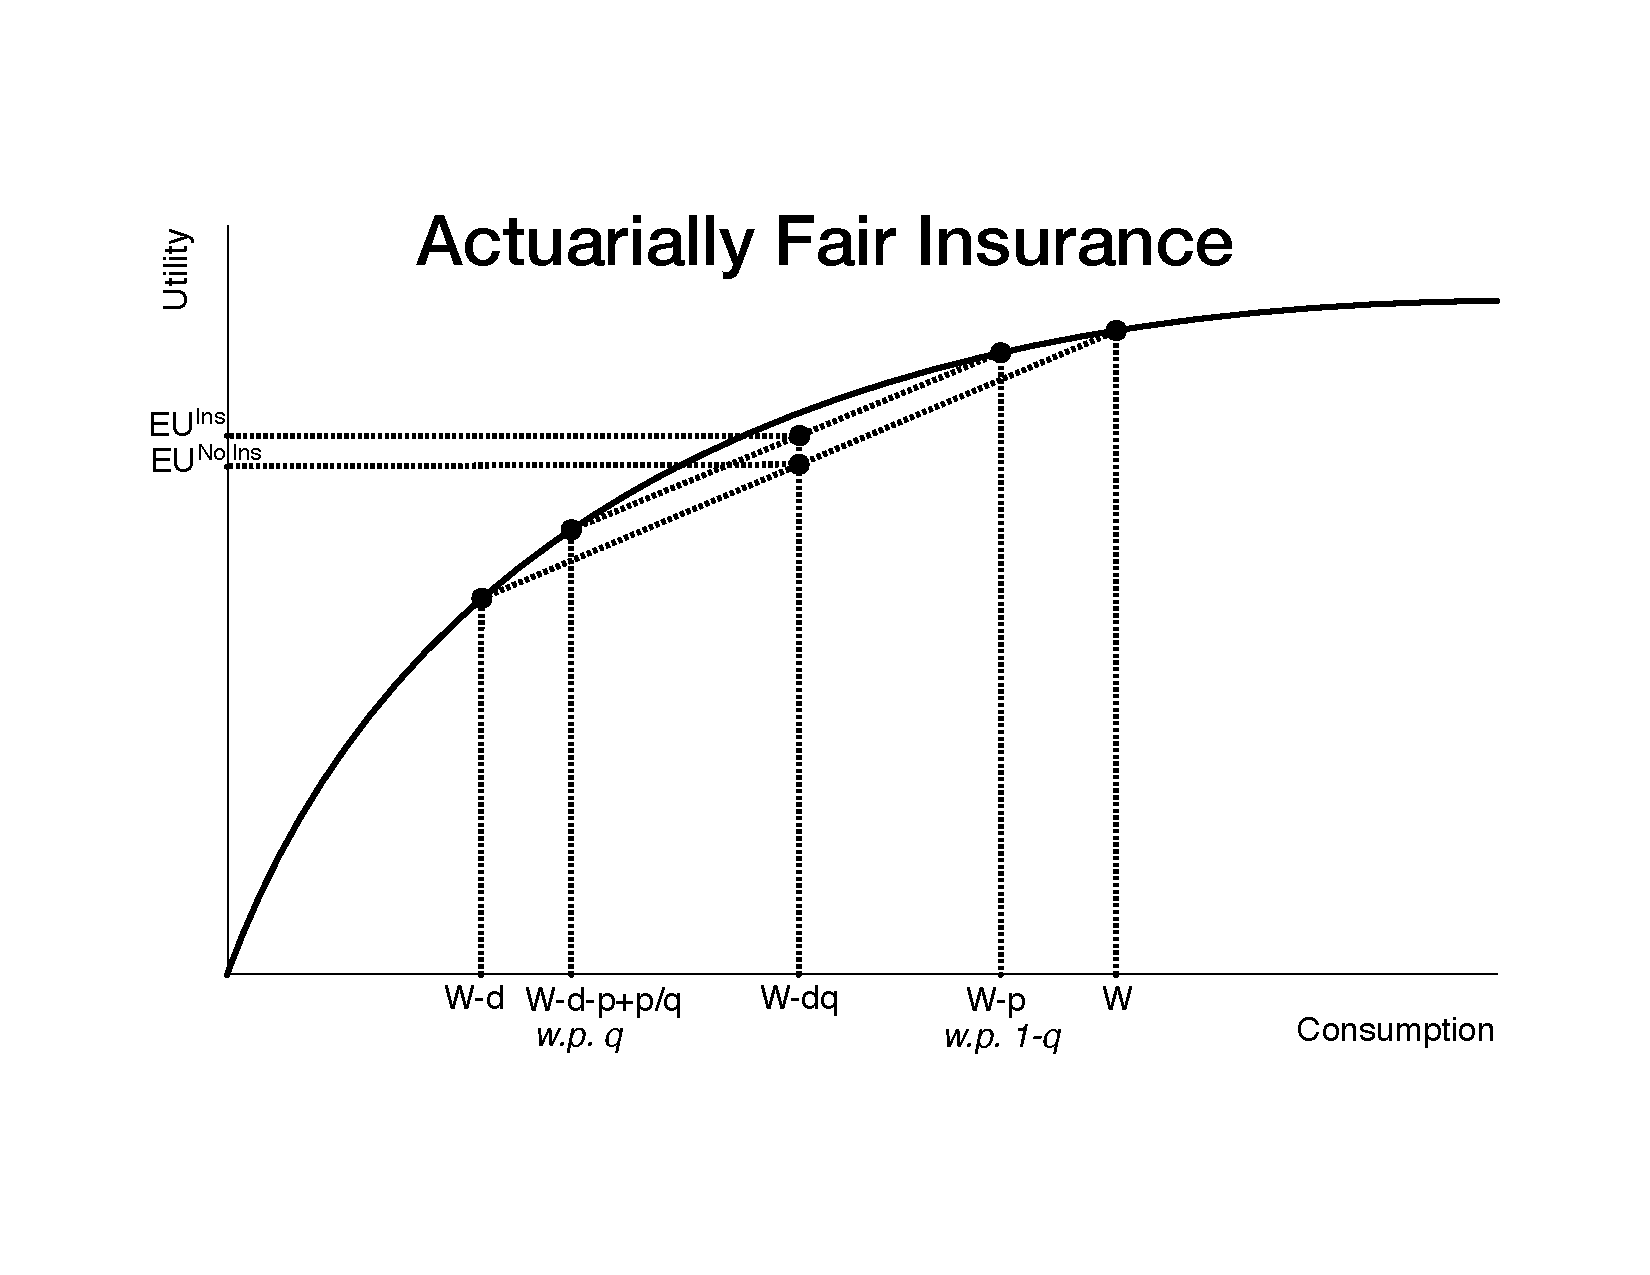
\includegraphics[width=10cm]{images/insurance_expected_utility.pdf}
    \end{center}
    \begin{itemize}
      \item The expected utility with actuarially fair insurance: $EU^{\text{Ins}} = (1-q)U(W-p) + qU(W-d-p+p/q)$
      \item If an individual can choose $p$ to maximize expected utility, and they are risk averse:
        \begin{align*}
          \frac{\partial EU^{\text{Ins}}}{\partial p} &= 0\\
          p &= d\cdot q \tag*{Premium = Expected Damage}\\
          b &= d \tag*{Benefit = Damage}
        \end{align*}
      \item A risk-averse individual will choose actuarially fair \textit{full} insurance.
    \end{itemize}
    \begin{center}
      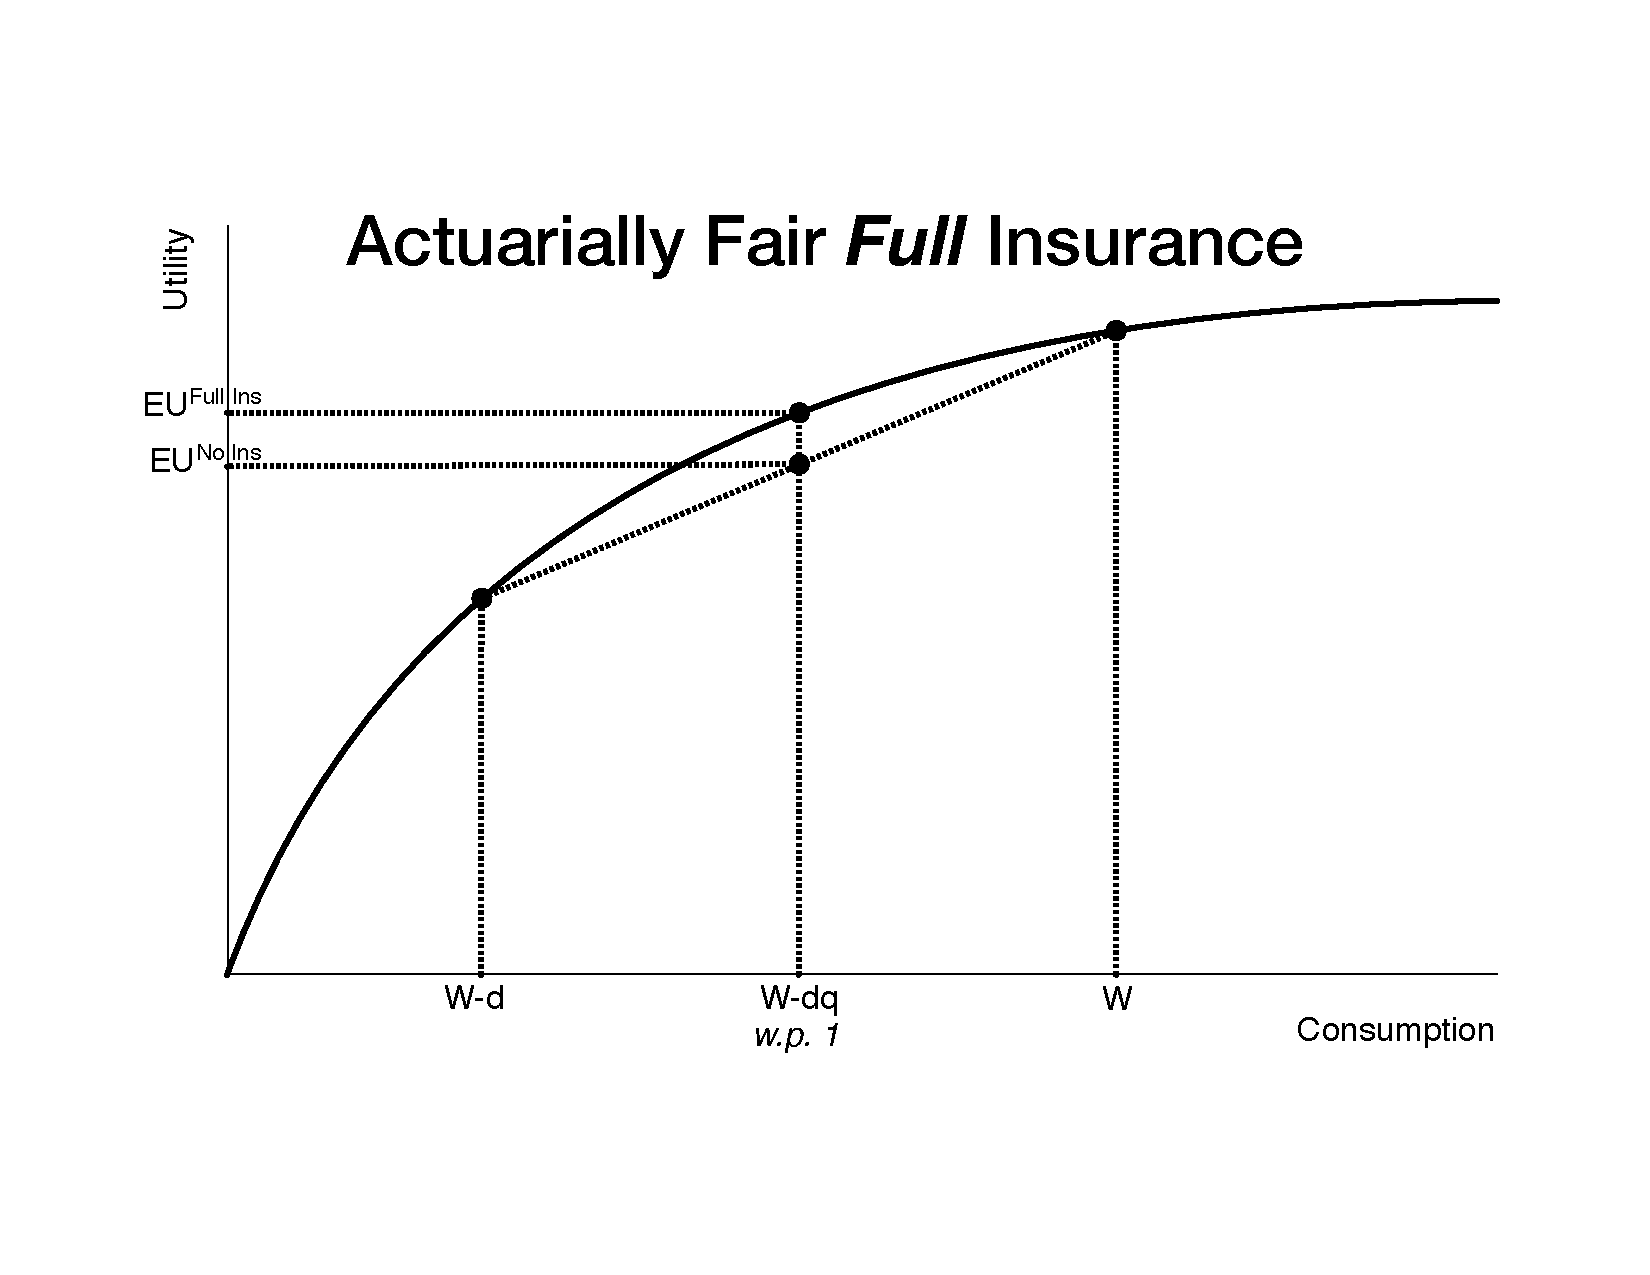
\includegraphics[width=10cm]{images/full_insurance_expected_utility.pdf}
    \end{center}
    \begin{itemize}
      \item The overall consumption in both states is $W - d\cdot q$, meaning $EU^{\text{Full Ins}} = U(W-dq)$
      \item The maximum that an individual is willing to pay is  $p'$ such that $EU^{\text{No Ins}} = U(W - p')$ (essentially, they have to be at least indifferent to buying insurance with premium $p'$ and remaining uninsured). If $p' > dq$, then the individual will be fully insured, else they will be partially insured at $p'$.
    \end{itemize}
  \end{problem}
  \begin{problem}{Social Insurance}
    \begin{itemize}
      \item The government provides social insurance for a range of events:
        \begin{itemize}
          \item Social Security (money in retirement)
          \item Unemployment Insurance (job loss)
          \item Disability Insurance
          \item Workers' Compensation (for job accidents)
          \item Medicare (healthcare for the old)
          \item Income supports (poverty)
        \end{itemize}
      \item The growth in government in the past 100 years was primarily due to the growth in social insurance.
    \end{itemize}
    However, as we saw in the insurance theory section, we might wonder why the government would get involved in creating social insurance.\\

    The answer is \textbf{asymmetric information}.
    \begin{description}
      \item[Case 1 --- Symmetric Information:] Insurance companies and individuals can observe types.
        \begin{itemize}
          \item If this is allowed, then the insurance companies will offer two actuarially fair policies, $(p_s, b_s = p_s/q_s)$ for sick people, and $(p_h, b_h = p_h/q_h)$ for healthy people.
          \item Each type $i$ will choose to buy full insurance, $p_i = dq_i$ and $b_h = b_s = d$.
          \item Private insurance does not equalize incomes across types, only within types: each consumes $W - dq_i$ in each state.
          \item Pre-existing conditions will lead to inequality in insurance premia and welfare, but no market failure.
        \end{itemize}
      \item[Case 2 --- Asymmetric Information:] Insurance companies cannot observe or price different types, but individuals know their risk.
        \begin{itemize}
          \item If insurance companies offer the same two policies but everyone wants to buy the healthy insurance with lower premia, the insurance company will make losses.
          \item Insurance companies could offer a single full insurance contract at the \textit{average} actuarially fair price, which is a bad deal for low risk people and they may not buy.
          \item \textbf{Adverse selection} occurs when individuals know more about their risk level than the insurer, meaning higher risk people are more likely to buy insurance.
          \item Adverse selection can cause the insurance market to unravel in a death spiral, leading to no insurance contract even if everyone would benefit from full insurance.
        \end{itemize}
    \end{description}
    \begin{itemize}
      \item The private market can avoid a death spiral in two ways:
        \begin{description}
          \item[Pooling:] The insurance companies may be able to offer one contract that is a good deal for sick people but mediocre (but still net good) for healthy people.
          \item[Separating:] Insurance companies offer one full insurance contract for the sick and one partial insurance contract for healthy, which each type self-selects into. This equilibrium is inefficient as the healthy are still under-insured.
        \end{description}
      \item The government's solution is to require insurance.
        \begin{itemize}
          \item This leads to redistribution from the healthy to the sick.
          \item If society views health as primarily determined by luck, such redistribution can receive strong public support.
          \item All OECD countries have universal health insurance (and the United States is quite close to universal health insurance)
        \end{itemize}
    \end{itemize}
    There are other reasons for public insurance too:
    \begin{description}
      \item[Redistribution:] May not be the side effect of addressing adverse selection, but the motivating rationale.
      \item[Externalities:] Lack of insurance can be a cause of illness for me, thereby exerting a negative externality.
      \item[Behavioral Mistakes:] Individuals may be myopic or inattentive, leading them to not insure themselves.
      \item[Administrative Costs:] Administrative burden tends to be lower in public insurance than private insurance.
    \end{description}
    However, there is the problem of \textbf{moral hazard}, where people take adverse actions in response to taking on an insurance contract. 
    \begin{itemize}
      \item Reduced precaution against entering the adverse state (i.e., driving more recklessly when one has auto insurance)
      \item Increased odds of staying in the adverse state (remaining unemployed longer after one receives unemployment insurance)
      \item Increased expenditures when in the adverse state (overspending on healthcare procedures when one has health insurance)
    \end{itemize}
    Social insurance systems should partially, but not fully insure individuals (to properly balance consumption smoothing benefits with moral hazard costs).
  \end{problem}
  \begin{problem}{The Retirement Problem}
    During earning years, people save up money via working in order to smooth their consumption, and wealth tends to peak right around retirement age --- if people live for too long, however, their wealth might be ``used up'' before they die.
    \begin{center}
      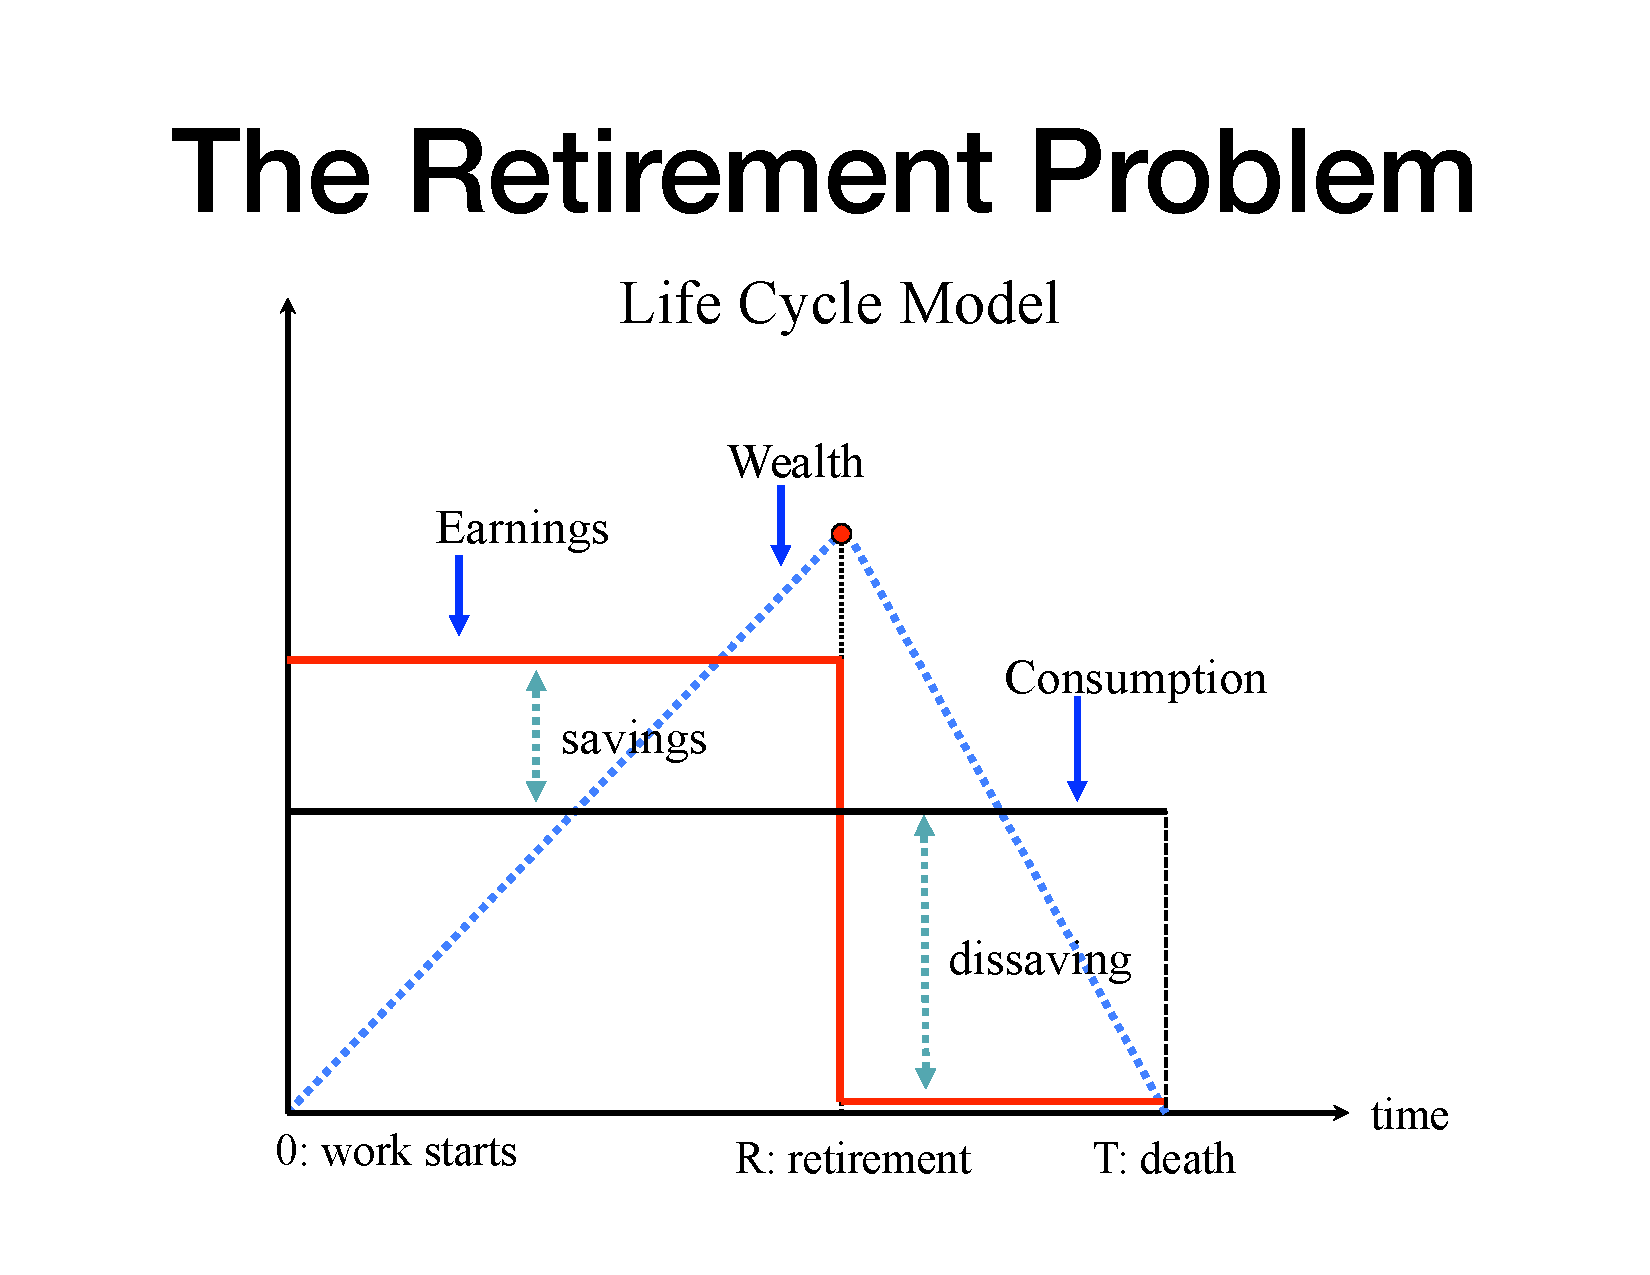
\includegraphics[width=10cm]{images/retirement_problem.pdf}
    \end{center}
    Before the advent of the welfare state (starting in the late 1800s, then ramping up in the 1930s and 40s), people above the age of 65 worked a lot more than they do now.
    \begin{center}
      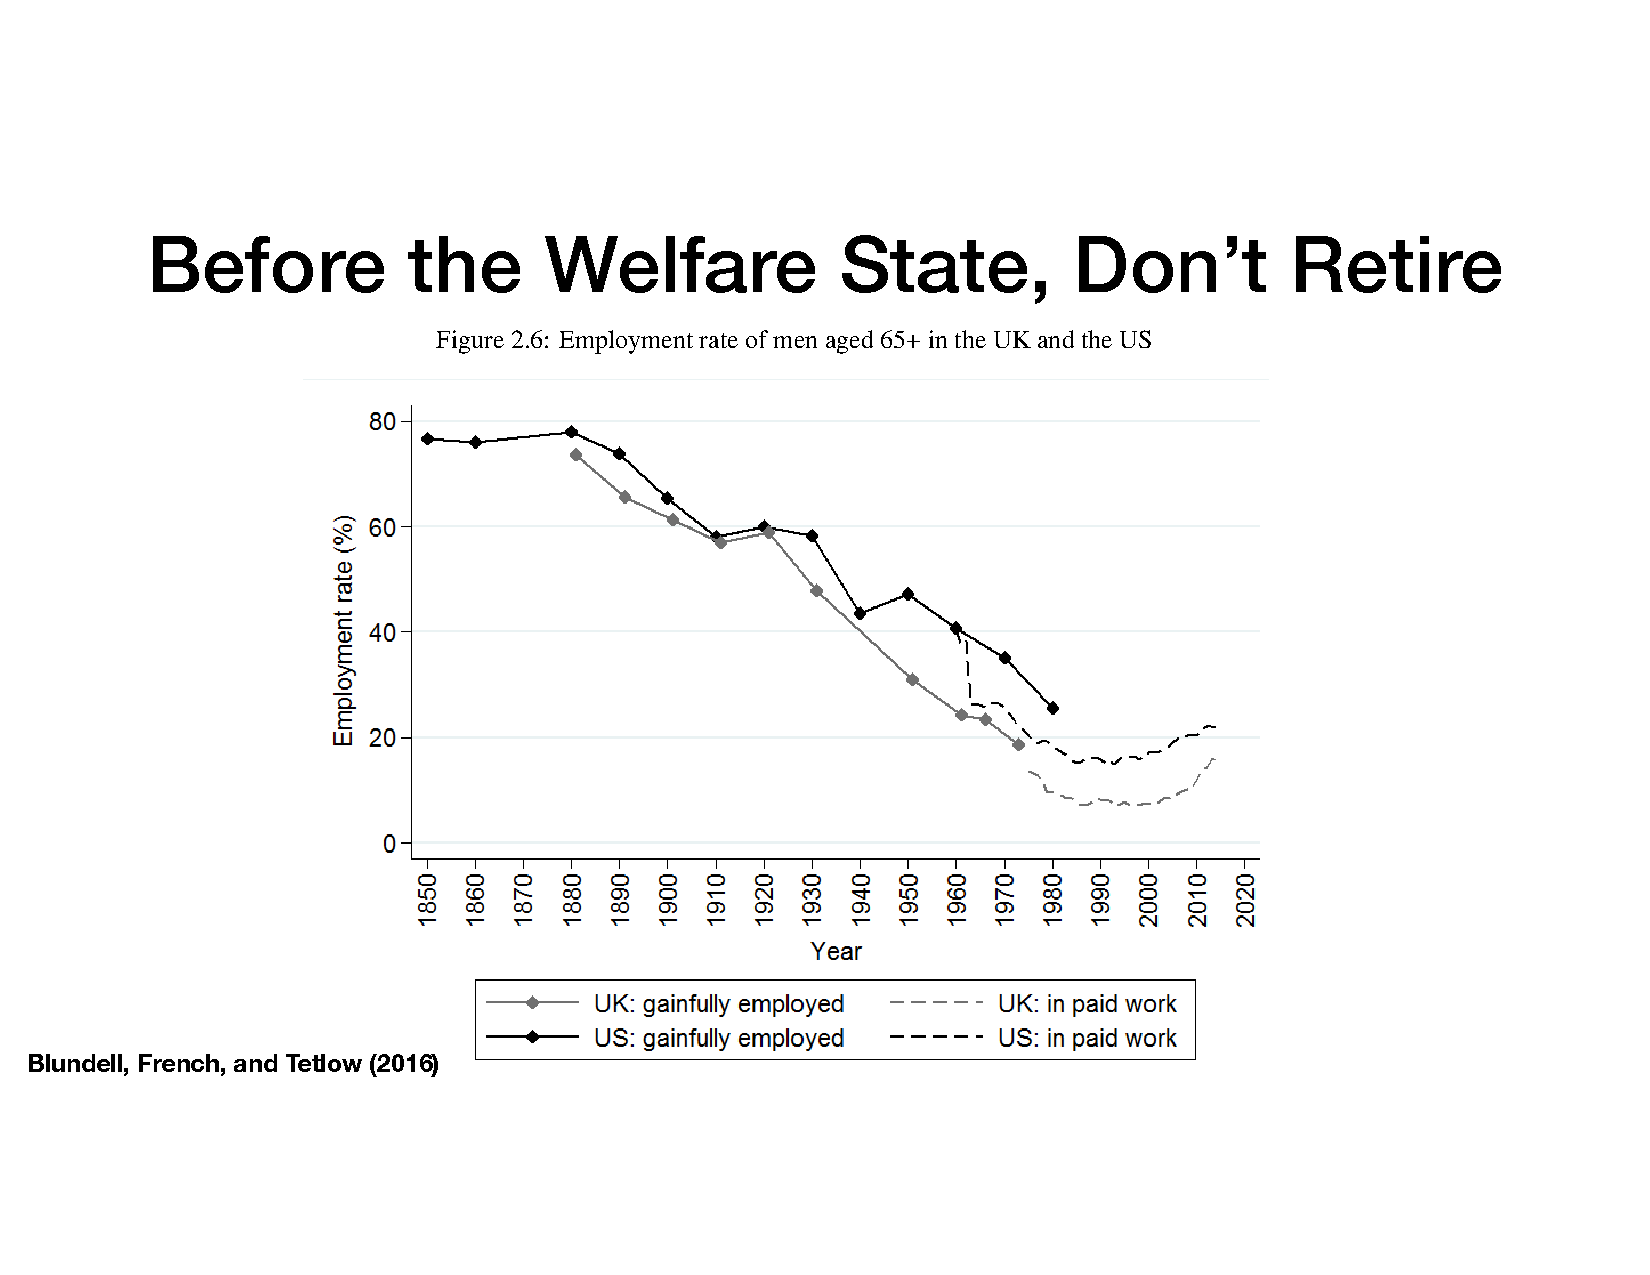
\includegraphics[width=\textwidth]{images/working_hours.pdf}
    \end{center}
    \begin{itemize}
      \item Most OECD countries provide government-funded retirement programs around 5--10\% of GDP.
      \item Individuals pay payroll taxes while working and receive annuity until death (annuities are essentially equivalent to insurance against living too long) 
      \item It's no longer working kids who take care of you in old age, but all the workers in the country.
      \item In the U.S., public retirement is called \textbf{Social Security}, and is the largest single expenditure of the federal government.
    \end{itemize}
  \end{problem}
  \begin{problem}{Social Security Details}
    The payroll tax is a 12.4\% tax on earnings up to a cap of \$160,000.\newline

    Workers who have worked and paid for 40 quarters and are at least 62 years old are eligible.\newline

    The annuity payment is a function of the person's 35 highest earning years, where each month's earnings are expressed in today's dollars (AIME: average indexed monthly earnings).\newline

    The function for PIA in terms of AIME is expressed as follows:
    \begin{align*}
      P(I) &= \begin{cases}
        0.9I,& I \leq 895\\
        806 + 0.32(I - 895),& 895 < I \leq 5397\\
        2246 + 0.15(I - 5397),& 5397 < I \leq 6316
      \end{cases}
    \end{align*}
    One way in which social security is regressive is that rich people tend to live longer than poor people, and will generally receive more in benefits. One of the risks with increasing the retirement age is that doing so may lock out lower income people.\newline

    Sources of retirement income:
    \begin{enumerate}[(1)]
      \item Social Security: for 2/3 of retirees, SS is >50\% of income, 1/3 of elderly households depend almost entirely on SS.
      \item Homeownership: 75\% of elderly households are homeowners.
      \item Pensions: 40--45\% of elderly US households have pensions:
        \begin{itemize}
          \item Defined Benefit pensions: employer carries full risk.
          \item Defined Contribution pensions: 401(k)s, employee carries risk.
        \end{itemize}
      \item Savings: about 10\% of retirees have significant extra savings.
    \end{enumerate}
    Most of the wealth in the bottom 90\% of retirees is housing + pensions - debts (mortgage, consumer credit, student loans).
  \end{problem}
  \begin{problem}{Types of Programs}
    There are two primary forms of retirement programs:
    \begin{itemize}
      \item Unfunded (pay-as-you-go): Benefits of current retirees are paid out of contributions from current workers (also known as a generational link).
        \begin{center}
          current benefits = current contributions
        \end{center}
      \item Funded: worker contributions are invested in financial assets and will pay for benefits when they retire.
        \begin{center}
          current benefits = past contributions + market returns on past contributions
        \end{center}
      \item Social Security has traditionally been unfunded, but the trust fund helps finance current benefits out of treasury bonds it purchases with payroll taxes.
      \item Private retirement plans are funded.
    \end{itemize}
  \end{problem}
  \begin{problem}{Evaluating Social Security}
    Recall that optimal social insurance balances consumption-smoothing benefits with moral hazard costs.\newline

    People tend not to smooth their own consumption for two main reasons:
    \begin{itemize}
      \item Adverse selection in the annuities market:
        \begin{itemize}
          \item People with shorter life expectancy tend to be less likely to buy private annuities, increasing their price.
          \item Market could unravel.
        \end{itemize}
      \item Behavioral mistakes:
        \begin{itemize}
          \item people tend not to save for their retirement due to myopia, inattention, self-control issues, etc.
          \item Social Security's popularity suggests that people understand their own failure to align savings intentions with savings actions.
        \end{itemize}
    \end{itemize}
    We model this via a two period life-cycle model with $c_1$ while working and $c_2$ in retirement.
    \begin{itemize}
      \item Period 1 budget constraint: $c_1 + s = W$, where $W$ equals earnings.
      \item Period 2 budget constraint: $c_2 = s(1+r)$, where $r$ is the interest rate.
      \item Our intertemporal budget constraint:
        \begin{align*}
          c_1 + c_2/(1+r) = W
        \end{align*}
      \item We want to find the following:
        \begin{align*}
          \max_{c_1,c_2}u(c_1) + \delta u(c_2)
        \end{align*}
        such that $c_1 + c_2/(1+r) = W$, where $\delta\in[0,1]$ refers to the discount factor.
    \end{itemize}
    \begin{center}
      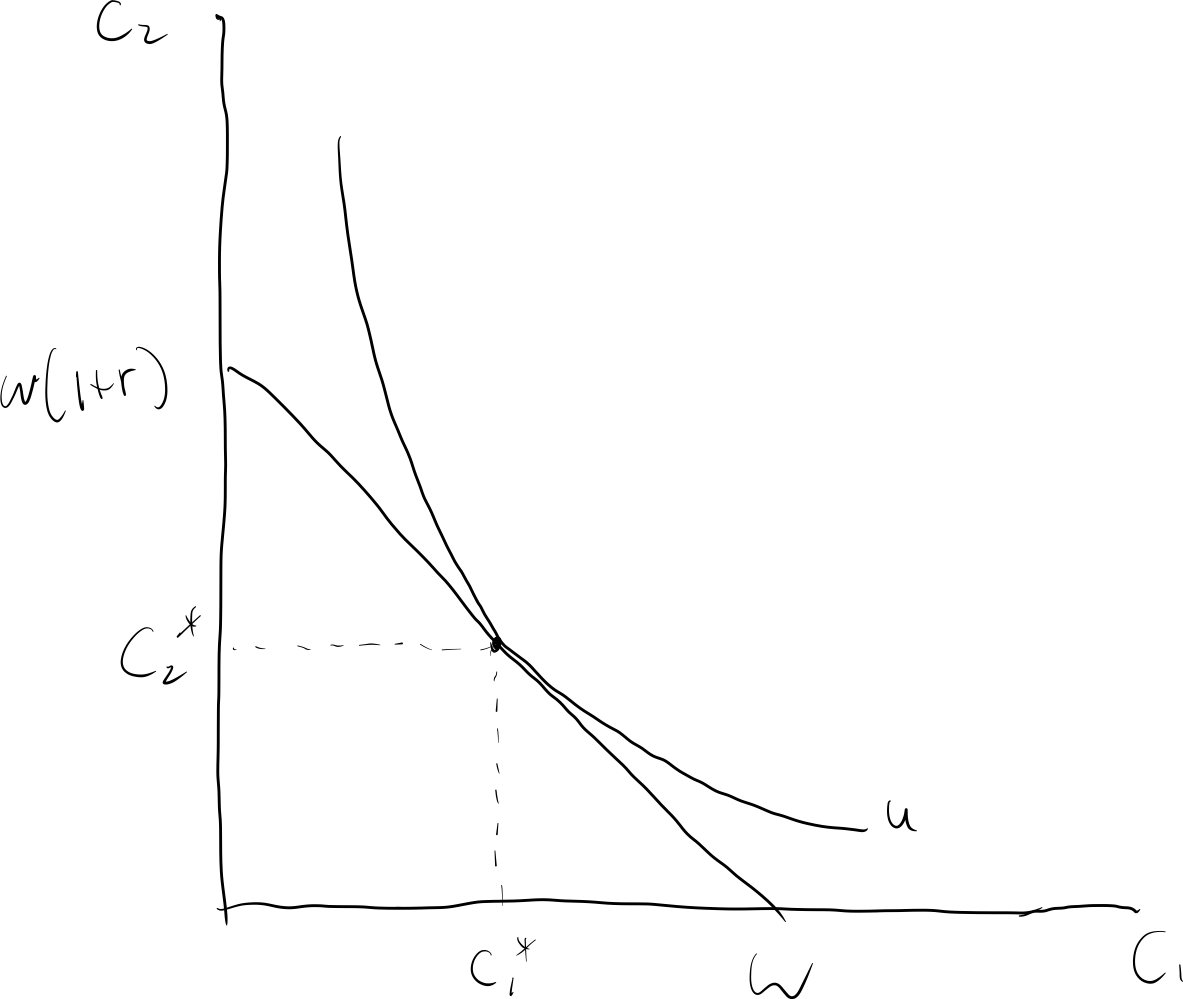
\includegraphics[width=7cm]{images/utility_max_retirement.png}
    \end{center}
    \begin{itemize}
      \item The solution is as follows:
        \begin{align*}
          MRS_{c_1,c_2} &= \frac{u'(c_1)}{\delta u'(c_2)}\\
                       \frac{u'(c_1)}{\delta u'(c_2)} &= \frac{P_1}{P_2}\\
                                                      &= (1+r)\\
                       u'(c_1) &= \delta (1+r) u'(c_2)
        \end{align*}
      \item Standard assumption: $\delta = \frac{1}{1+r}$
        \begin{align*}
          \frac{u'(c_1)}{u'(c_2)(1+r)} &= (1+r)\\
          u'(c_1) = u'(c_2)\\
          c_1^* &= c_2^*\\
          s^* &= W - c_1^*
        \end{align*}
      \item (Extreme) Myopia: $\delta = 0$
        \begin{align*}
          c_1 &= W\\
          c_2 &= 0
        \end{align*}
    \end{itemize}
    Introduce a social security program:
    \begin{itemize}
      \item Forced savings tax $\tau$ equal to the amount saved by standard savers
      \item Retirement benefit: $b = \tau(1+r)$.
      \item This tax does not affect the myopic saver (0\% crowd-out of private savings), and fully crowds out the rational saver.
    \end{itemize}
    \begin{center}
      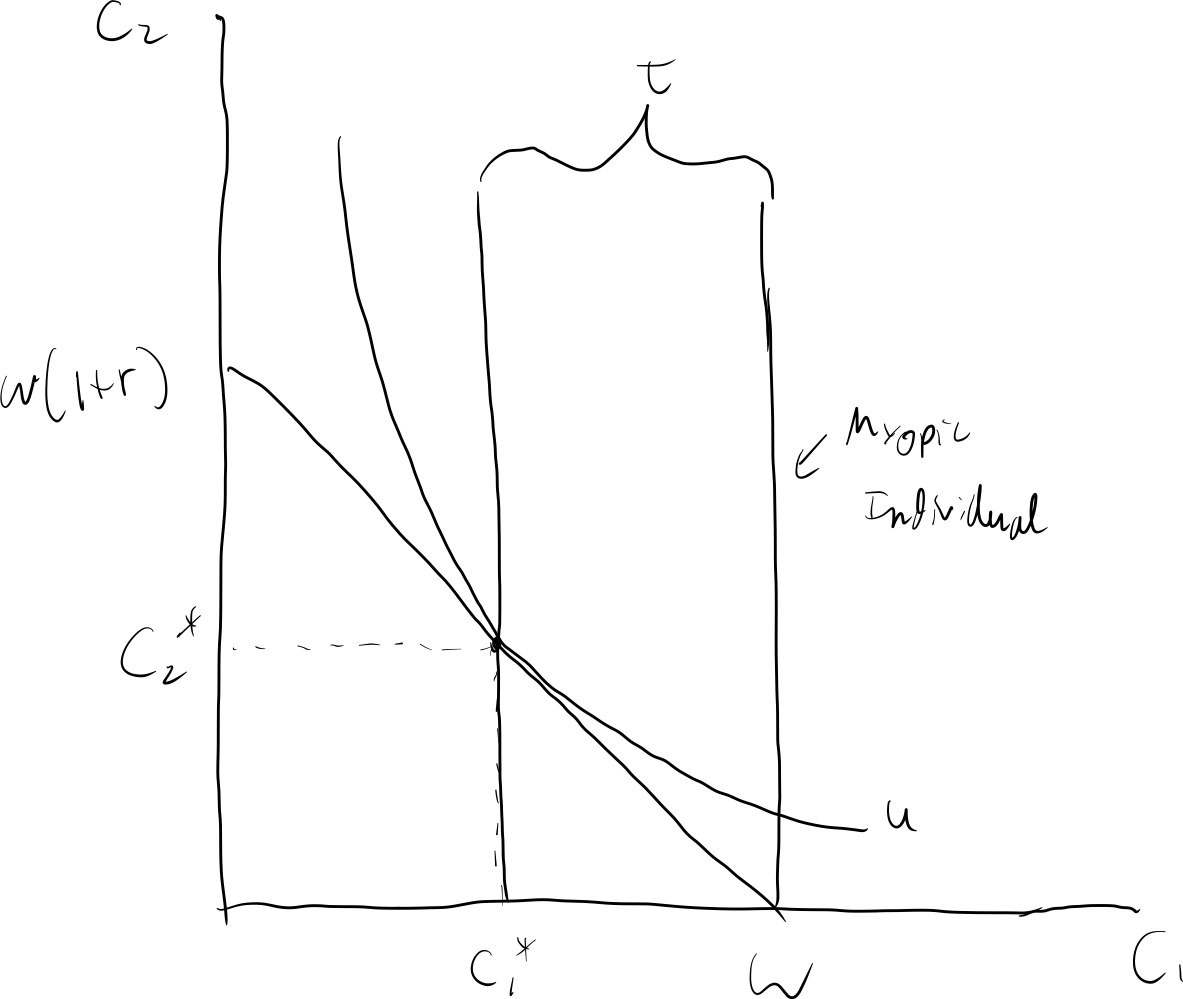
\includegraphics[width=7cm]{images/retirement_myopia.png}
    \end{center}
    Evidence suggests that social security has about 30--40\% crowd-out, implying that people are predominantly myopic.\newline

    Consumption, on average, drops substantially for all quartiles of wealth, except for those who also had top quartile income.\newline

    However, social security has likely contributed to a substantial drop in poverty for the elderly.
  \end{problem}
  \begin{problem}{Moral Hazard}
    \begin{itemize}
      \item Key efficiency cost of SS is the moral hazard of inducing workers to retire early.
      \item Benefits available at Early Eligibility Age (62), before Full Benefit Age (67).
      \item If a 62 year old worker works until 63, three things happen:
        \begin{itemize}
          \item Cost 1: One extra year of payroll tax.
          \item Cost 2: One year less of SS benefits.
          \item Benefit: Higher adjusted SS benefit (8\% extra per year of delay)
        \end{itemize}
      \item The adjustment is actuarially fair if the benefit outweighs the two costs perfectly (as is basically true in the United States)
      \item Two big issues:
        \begin{itemize}
          \item EEA might encourage early retirement.
          \item Non-actuarially fair benefits may create a large implicit tax on work.
        \end{itemize}
    \end{itemize}
    Retirement rate increases substantially around EEA, suggesting substantial moral hazard.\newline

    The actuarial adjustment among most countries tends to disincentivize work relative to the United States.
  \end{problem}
  \begin{problem}{Current Problems and future outlook of Social Security}
    \begin{itemize}
      \item Increase in life expectancy at retirement.
      \item Decrease in birth rates (fewer workers in the generational link)
      \item Increasing number of elderly per working age adult.
      \item Slower productivity growth since 1970.
    \end{itemize}
    Social Security requires adjusting taxes and/or benefits to remain in balance. The first set of reforms were implemented in 1983, and attempted to solve the SS budget shortfall via the following:
    \begin{itemize}
      \item Increased payroll taxes to create the trust fund.
      \item Increased retirement age for full benefit (from 65 to 67)
    \end{itemize}
    The trust fund peaked recently, and will be exhausted in 2034 --- taxes will cover 75\% of promised benefits.\newline

    Reform options:
    \begin{enumerate}[(1)]
      \item Increase payroll tax now to 15.84\%, or increase payroll tax to 16.55\% in 2035
      \item Increase base of wages (immigration, tax wages above 160K)
      \item Reduce benefits:
        \begin{itemize}
          \item Index retirement age to life expectancy (likely regressive)
          \item Index benefits to chain-price CPI rather than CPI
          \item Make benefits taxable for income tax
        \end{itemize}
      \item Means-testing
      \item Invest trust fund in higher-yield assets
      \item Privatization (very unpopular)
    \end{enumerate}
  \end{problem}
  \begin{problem}{Unemployment Insurance}
    \begin{itemize}
      \item Unemployment Insurance, like other social insurance programs, is triggered by an adverse event (namely, involuntary job loss).
      \item UI tends to spend about \$20--30 billion/month in normal times.
      \item Plays a role in macroeconomic stabilization --- Congress often extends unemployment insurance to stabilize the economy.
      \item Need to balance consumption smoothing benefits with moral hazard cost.
    \end{itemize}
    Different countries tend to have different structures for the generosity of unemployment insurance and length of term.
  \end{problem}
  \begin{problem}{Optimal UI Theory}
    We want to define UI as that which maximizes utility.
    \begin{align*}
      EU &= (1-p)u(c_e) + pu(c_u)\\
         &= (1-p)u(w-t) + pu(b)
    \end{align*}
    \begin{itemize}
      \item $p$: probability of being unemployed
      \item $c_e$: consumption when employed
      \item $c_u$: consumption while unemployed
      \item $w$: wage while working
      \item $t$: taxes used to finance program
      \item $b$: unemployment insurance benefit
    \end{itemize}
    The actuarially fair taxes are as follows:
    \begin{align*}
      (1-p)(t) &= (p)(b)\\
      t &= \frac{p}{1-p}b
    \end{align*}
    If there is no moral hazard, then $p$ is not affected by $b$:
    \begin{align*}
      EU &= (1-p(b))u\left(w-\frac{p}{1-p}b\right) + pu(b)
    \end{align*}
    The optimal benefit $b^*$ is that where $c_u = c_e$ (i.e., full insurance with no moral hazard).\newline

    However, if there is moral hazard, and $p$ is a function of $b$, we would have to change the expected utility as follows:
    \begin{align*}
      EU &= (1-p)u\left(w - \frac{p(b)}{1-p(b)}b\right) + pu(b)
    \end{align*}
    The optimal benefit now is that which satisfies the following equation:
    \begin{align*}
      \frac{u'(c_u) - u'(c_e)}{u'(c_e)} &= \frac{\varepsilon_{p,b}}{p-1}\\
       &= \frac{1}{1-p}\frac{b}{p}\cdot\frac{dp}{db}
    \end{align*}
    where $\varepsilon_{p,b}$ denotes the elasticity of the unemployment rate with respect to benefits. This equation sets the consumption smoothing benefit from UI equal to the moral hazard cost.\newline

    The implication of this equation is that partial insurance is optimal: $0 < c_u < c_e < w$.\newline

    It is difficult to estimate the optimal benefit using the previous formula: consumption smoothing benefits require knowledge of the utility function, wages, and other savings that are unobservable.\newline

    To do this, Raj Chetty uses a Taylor approximation: $u'(c_u) - u'(c_e) = u''(c_e)(c_u - c_e)$.
    \begin{align*}
      \frac{\varepsilon_{p,b}}{1-p} &= \frac{u'(c_u) - u'(c_e)}{u'(c_e)}\\
                                    &\approx \frac{u''(c_e)(c_u - c_e)}{u'(c_e)}\\
                                    &= \underbrace{\left(-\frac{u''(c_e)}{u'(c_e)}c_e\right)}_{\text{\tiny coeff. of relative risk aversion}}\left(\frac{c_e - c_u}{c_e}\right)\\
                                    &= \gamma \frac{\Delta c}{c_e}(b^*)
    \end{align*}
    It is possible to measure $\gamma$, $\varepsilon_{p,b}$, and consumption, meaning we can empirically find $b^*$.\newline

    This equation extends to models with arbitrary savings, borrowing constarints, private insurance, and leisure benefits of unemployment.
    \begin{problem}{Moral Hazard in Unemployment Insurance: Empirical Evidence}
      Since, in the United States, unemployment policy differs by state, we have quasi-experimental variation.\newline

      Meyer (1990) finds that $\varepsilon_{p,b} \approx 0.5$, average.
    \end{problem}
    \begin{problem}{Consumption Smoothing in Unemployment: Empirical Evidence}
      Consumption falls by 10--15\% when people lose their job.\newline

      A 10 percentage point increase in the UI replacement rate causes a 2.8\% reduction in the rate of consumption drop.
      \begin{itemize}
        \item The replacement is much less than one to one, because UI tends to crowd out other self-insurance behaviors: spouses work less and individuals save less.
      \end{itemize}
    \end{problem}
    The current consensus is that the optimal UI replacement rate is around 50\%, paid in a constant path.
  \end{problem}
  \begin{problem}{Disability Insurance}
    \begin{itemize}
      \item Disability is close to retirement: some people become unable to work before old age.
      \item All rich countries offer a form of public disability insurance --- almost always linked to the public retirement system.
      \item Key issue that makes disability different from UI is \textit{screening}.
      \item Moral hazard: incentive to exaggerate or make fraudulent claims.
      \item Screening challenge: back injuries and mental health conditions especially.
      \item Audits of Bureau of Disability Insurance assessments reveal substantial rates of error.
        \begin{itemize}
          \item Oftentimes there are different acceptance thresholds for men and women.
          \item Suggests that disability insurance applications should be gender blind or use machine learning algorithms. 
        \end{itemize}
      \item Disability Insurance has increased substantially over time. Two views:
        \begin{itemize}
          \item Lenient system leads to inefficiency.
          \item Program helping people with legitimate needs.
        \end{itemize}
    \end{itemize}
  \end{problem}
  \begin{problem}{Evidence and Optimality of Disability Insurance}
    Quasi-experimental evidence: Maestas, Mullen, and Strand (2013) exploit random variation in DI examiners' stringency, find that labor force participation would have been 28 percentage points higher without DI.\newline

    Meyer and Mok (2019) find that food and housing consumption fall by 24\% with disability and 2/3 never return to work.\newline

    Evidence suggests that current DI benefits may be too low.
  \end{problem}
  \begin{problem}{Workers' Compensation}
    WC is insurance for temporary injuries on the job, covers medical costs and approximately 2/3 of lost wages.\newline

    Meyer, Viscusi, and Durbin (1995) find that a 10\% increase in WC benefit raises out-of-work duration due to injury by 4\%.\newline

    There are not a lot of empirical studies on the consumption smoothing benefits of WC.
  \end{problem}
  \begin{problem}{Health Insurance: Overview}
    There are multiple problems with healthcare and health insurance in the United States:
    \begin{itemize}
      \item Cost: The United States spends almost twice the OECD average (and approximately the OECD average on \textit{just} private healthcare).
      \item Despite this spending, the United States has a higher than average mortality, especially impacting native-born Americans without a high school education.
      \item Additionally, the United States has a relatively high uninsurance rate.
      \item The life expectancy problem in the United States is also made worse because the United States does not have above-average risk factors.
    \end{itemize}
    Primary policies of other countries: mandated universal coverage.
    \begin{itemize}
      \item \textbf{Beveridge Model:} single-payer insurance with government-run hospitals, private care, or mix. Primarily used in Anglophone countries and Sweden
      \item \textbf{Bismarck Model:} all-payer rate setting, non-profit insurance companies, mandated participation, and private care. Primarily used in Northern Europe, Israel, and Japan.
    \end{itemize}
    Governments control cost and limit overutilization by regulating for cost-effectiveness, setting prices, or rationing care, as well as cost-sharing with customer (coinsurance).\\

    In the United States, the plurality of health insurance (49\%) comes from employers, and another 34\% of people get health insurance through public health insurance. Only 6\% of people buy individual coverage.
    \begin{itemize}
      \item Most full-time employees are offered insurance through their employer, who contracts with an insurance company.
      \item For insurers, workers at firms are a large risk pool that avoids adverse selection.
      \item Employees participate because compensation in the form of health insurance is not taxed. More than \$270 billion in taxes are forgone through this process.
      \item The ``employer contribution'' is actually fully incident on the employee (i.e., it comes out of lost wages).
        \begin{itemize}
          \item Other drawbacks include job lock (can't get health insurance on the private market).
        \end{itemize}
      \item Individuals can buy insurance directly from an insurer rather than through a group plan.
      \item Before Obamacare, this market was plagued by adverse selection (thanks to everyone who had group insurance subsidized via the tax code through their employer).
      \item Obamacare exchanges forbid price discrimination on the basis of pre-existing conditions and provide subsidies for buying individual insurance.
      \item Additionally, Obamacare expanded Medicaid to cover everyone under the poverty line and imposed a penalty on those who did not purchase insurance through the exchanges.
      \item However, after the Tax Cuts and Jobs Act (2017), the penalty was set to zero; many were worried about unraveling of the individual insurance market.
    \end{itemize}
  \end{problem}
  \begin{problem}{Health Insurance: Evaluation and Optimal Policy}
    The consumption-smoothing benefits of health insurance depend on the magnitude of the potential loss.
    \begin{itemize}
      \item Small shocks lead to small differences in marginal utility in the healthy and unhealthy states.
      \item Small predictable losses can be self-insured via saving.
    \end{itemize}
    The moral hazard from health insurance manifests in overconsumption because insured people pay only a fraction of healthcare costs when sick (also known as a co-pay or co-insurance). The question is the price elasticity of demand.\\

    In the late 1970s, the RAND corporation randomly assigned 6000 people different types of health insurance with different co-pays plans to study moral hazard. They found three key things:
    \begin{itemize}
      \item Contrary to popular belief, demand for medical care is somewhat price sensitive. Individuals in the free plan used 1/3 more healthcare than those paying 95\%. The researchers found an elasticity of $-0.2$.
      \item Lower co-pays did not lead to a significant improvement in a participant's health.
      \item For those who are chronically ill and could not easily cover co-pays, there was some deterioration in health.
    \end{itemize}
    For small health shocks, there are low benefits and some moral hazard, meaning we should avoid insuring them.\\

    For large, unpredictable shocks, there are high benefits and less moral hazard.\\

    These results suggest that the optimal health insurance has a high deductible (so patients bear a large share of cost initially) and full coverage for catastrophes.\\

    However, ACA exchange data shows that people dislike plans with high deductibles.
    \begin{itemize}
      \item Brot-Goldberg et al. (2017) show that high deductible plans lead to large and likely inefficient cuts in healthcare use.
    \end{itemize}
  \end{problem}
  \begin{problem}{Evaluation of Medicare and Medicaid}
    Medicare Part D (which covers prescription drugs) was not optimal: there is 100\% coinsurance between \$0 and \$275, 25\% coinsurance between \$275 and \$2510, 100\% coinsurance between \$2510 and \$5726, and then 7\% coinsurance above \$5726.\\

    A study on Medicare Part D found that many people clustered their total annual expenditure around where the 25\% coinsurance segment ended, near \$2500. The ACA changed the \$0 -- \$5726 bracket to be 75\% coinsurance.\\

    We can examine the direct effects of health insurance on health directly rather than looking at consumption-smoothing. However, merely comparing health outcomes for people who are on Medicaid vs. those who are not would yield biased results.\\

    Currie and Gruber (1996) used Medicaid expansions as quasi-experiment to evaluate the value of the program.
    \begin{itemize}
      \item Utilization increased: early prenatal care visits rose by more than 50\%
      \item Infant mortality declined by 8.5\% due to the expansions in Medicaid for pregnant women.
      \item Policy was highly effective, only \$1.4m/life saved (value of a statistical life is around \$10m)
    \end{itemize}
    Finklestein et al. (2012) used a Medicaid lottery to estimate causal effects of coverage, specifically in Oregon. Lottery losers were the control, while lottery winners were the treatment group. Expanding access to Medicaid led to
    \begin{itemize}
      \item higher healthcare utilization
      \item lower out-of-pocket medical expenditures and medical debt
      \item slightly better self-reported physical health, and large improvements in mental health
    \end{itemize}
    Using regression discontinuity, Card, Dobkin, and Maestas (2008) found that Medicare availability led to increased utilization and lower post-hospitalization mortality.
  \end{problem}
  \begin{problem}{Health Insurance Benefits}
    How do we reconcile the RAND result that found little impact on increased coverage on health? The studies examine different parts of the \textbf{health effectiveness curve}.
    \begin{itemize}
      \item Moving individuals from uninsured to some insurance leads to strong positive effects on health.
      \item Adding to generosity of insurance does not cause significant changes in health.
    \end{itemize}
    The United States leaves many uninsured, but provides overly generous care to the insured.
  \end{problem}
  \begin{problem}{Provider-Side Evaluation}
    Consider a model where payment for physician services is $P = \alpha + \beta \cdot c$, where $\alpha$ is a fixed payment while $\beta$ is payment proportional to physician costs $c$.\\

    Physician contracts are primarily of two types:
    \begin{itemize}
      \item \textbf{Fee for Service}: $\alpha = 0, \beta > 1$, no fixed payment for practice, but insurance company pays full cost of visits + surcharge.
      \item \textbf{Diagnosis-based Payment}: $\alpha > 0, \beta = 0$, varying payment by type and number of patients, but not by services rendered.
    \end{itemize}
    If a physician is compensated for all costs, it is in their interest to do lots of procedures even if they aren't cost-effective.\\

    The general trend has been toward higher $\alpha$ and lower $\beta$.
    \begin{itemize}
      \item The private market has shifted toward \textbf{Health Maintenance Organization (HMO) capitation} contracts, where the insurer pays a fixed amount per patient regardless of health costs.
      \item Kaiser physicians receive a flat payment per person enrolled based on age/gender.
      \item However, lower $\beta$ provides incentives for doctors to provide fewer services, and maybe even too few services.
      \item In 1983, Medicare moved from fee for services to diagnosis-based payment. Cutler (1993) found that this shift led to:
        \begin{itemize}
          \item Reduction on treatment intensity --- doctors place some weight on profits.
          \item No adverse impact on patient outcomes --- doctors under fee for service were practicing non-cost-effective service.
          \item Cost growth slowed dramatically in the first five years, but then accelerated as hospitals upcoded treatments.
        \end{itemize}
    \end{itemize}
  \end{problem}
  \begin{problem}{Inflation Reduction Act: Effects on Healthcare}
    Medicare and Medicaid have been instructed to negotiate down prices of 10 high-cost drugs,\\

    Fee imposed on companies that raise price of Rx drugs faster than inflation.\\

    Out of pocket spending capped at \$35/month.\\

    Medicare and Medicaid recipients can get all vaccines for free.\\

    Medicare Part D cost-sharing reforms:
    \begin{itemize}
      \item In 2024, copay above catastrophic threshold drops to 0\%
      \item Starting in 2024, out of pocket costs capped at \$2K/year.
    \end{itemize}
    Estimated effects of these policies is savings of \$115 billion over next 10 years.
  \end{problem}
  \section*{Taxation and Redistribution}%
  \begin{problem}{Motivations for Redistribution}
    The primary motivation for government intervention in the economy is for correcting market failures, as we had analyzed in the previous section.
    \begin{itemize}
      \item Taxes and subsidies for negative/positive externalities
      \item Funding public goods
    \end{itemize}
    These interventions attempt to move the market equilibrium \textit{toward} the Utility Possibilities Frontier.\\

    Meanwhile, the objective of taxation and redistribution is to move \textit{along} the Utility Possibilities Frontier. However, there is a potential cost --- using taxes and transfers may move the market equilibrium outcome away from the Utility Possibilities Frontier.
  \end{problem}
  \begin{problem}{Labor and Capital Income}
    Individuals derive pre-tax income from \textit{labor} and \textit{capital}:
    \begin{align*}
      z &= wl + rk
    \end{align*}
    where $w$ is the wage, $l$ is the labor supply (in hours), $k$ is capital, and $r$ is the rate of return on capital.\\

    Labor income inequality is due to differences in:
    \begin{itemize}
      \item Work abilities reflected in $w$ (education, experience, talent, physical ability, etc.)
      \item Work effort reflected in $l$ (hours in work)
      \item Institutions (minimum wages, unions, etc.)
      \item Social norms (such as household division of labor) and discrimination (race and gender discrimination)
    \end{itemize}
    Capital income inequality is due to differences in:
    \begin{itemize}
      \item total capital stock $k$ (due to past saving and inheritance)
      \item rates of return $r$
    \end{itemize}
    In the aggregate, $wl$ makes up about $75\%$ of $z$, while $rk$ makes up about $25\%$ of $z$.\\

    The capital stock is about 400--500\% of $z$, with a rate of return $r$ of around $6\%$.
  \end{problem}
  \begin{problem}{Empirical Facts about US Income Inequality}
    \begin{center}
      Fact 1: Top income share is U-shaped, but has leveled off in the past decade.\\
      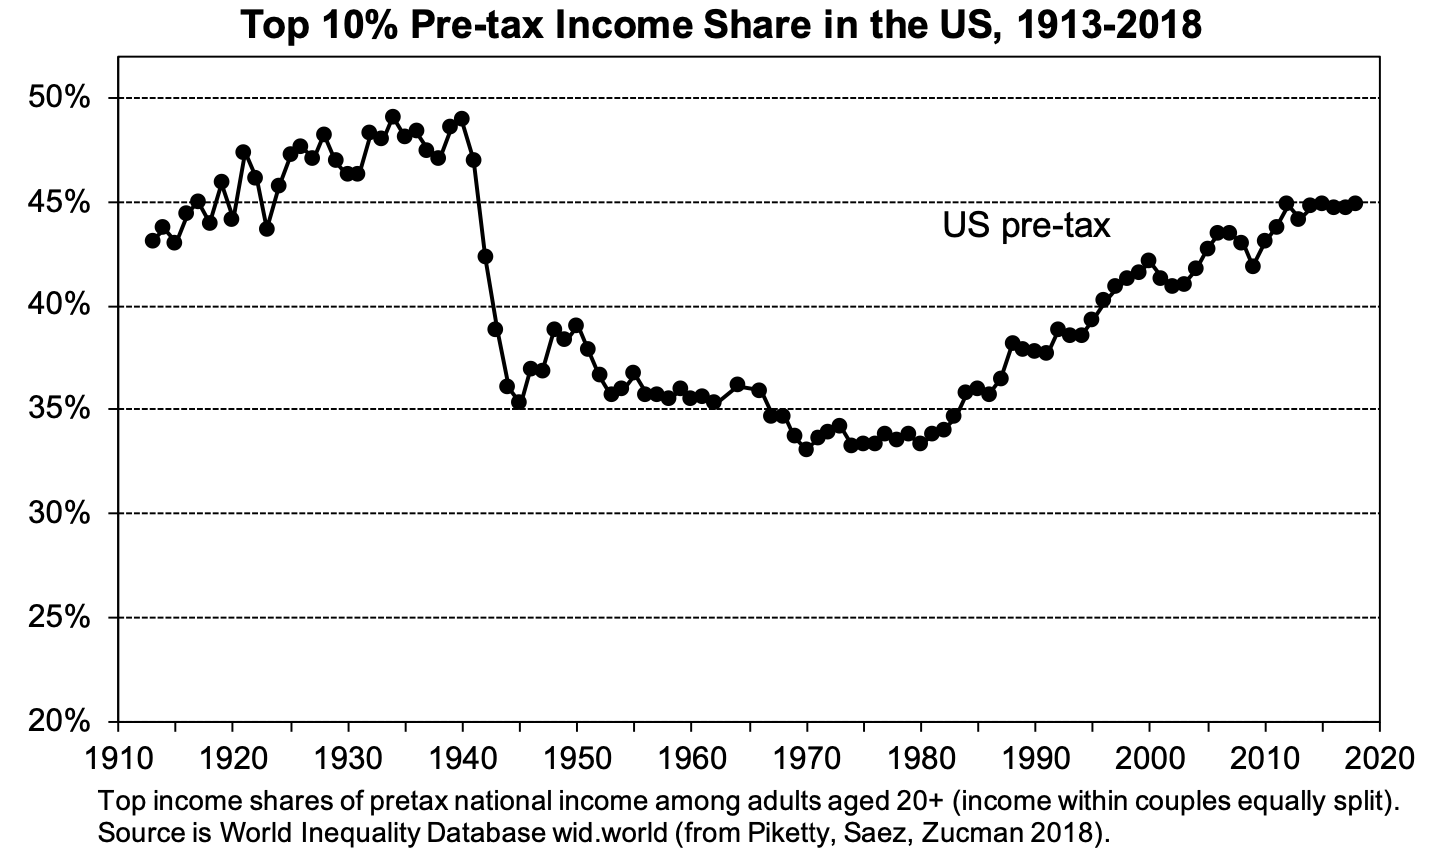
\includegraphics[width=0.8\textwidth]{images/pretax_income.png}
    \end{center}
    \begin{center}
      Fact 2: Income stagnation at the bottom of the income distribution.\\
      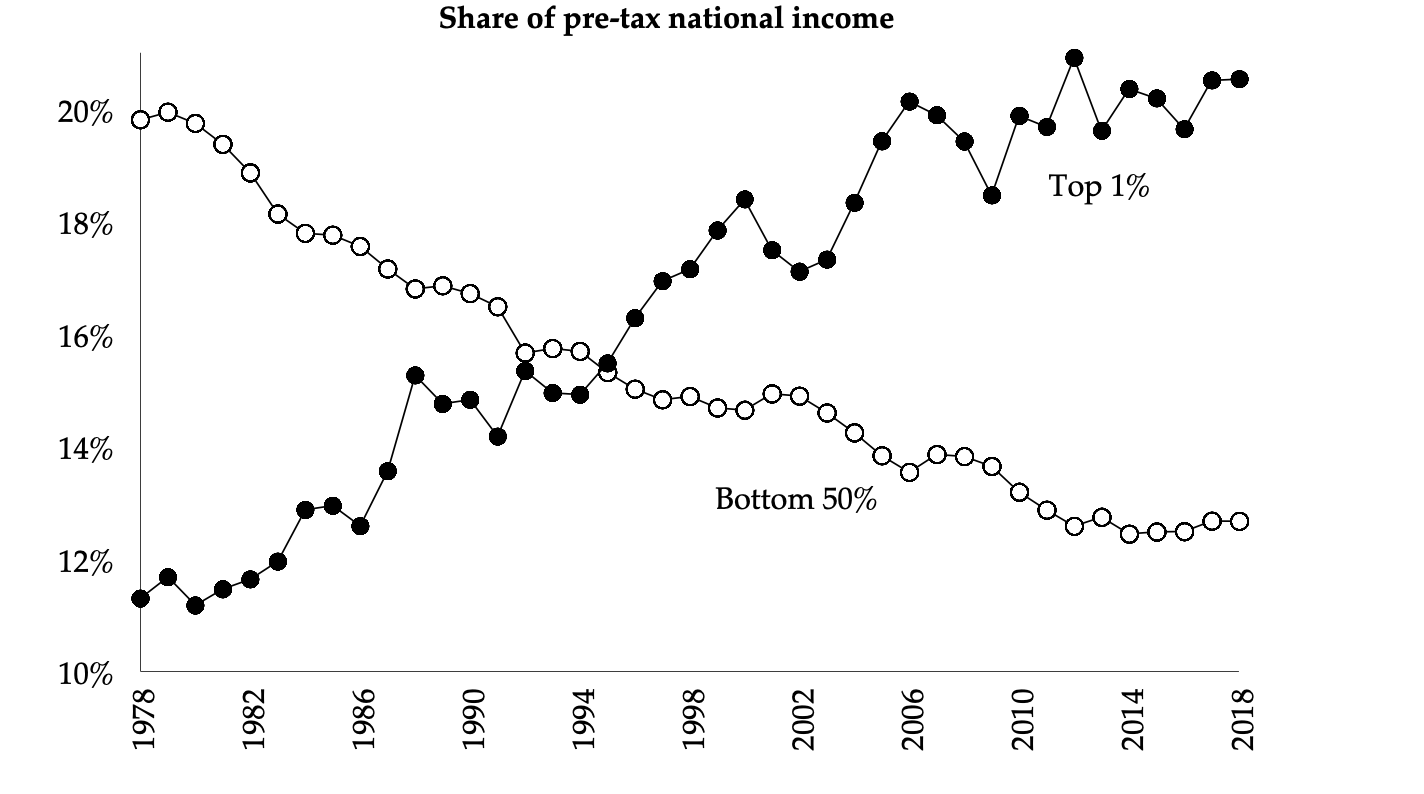
\includegraphics[width=0.8\textwidth]{images/bottom_stagnation.png}\\
      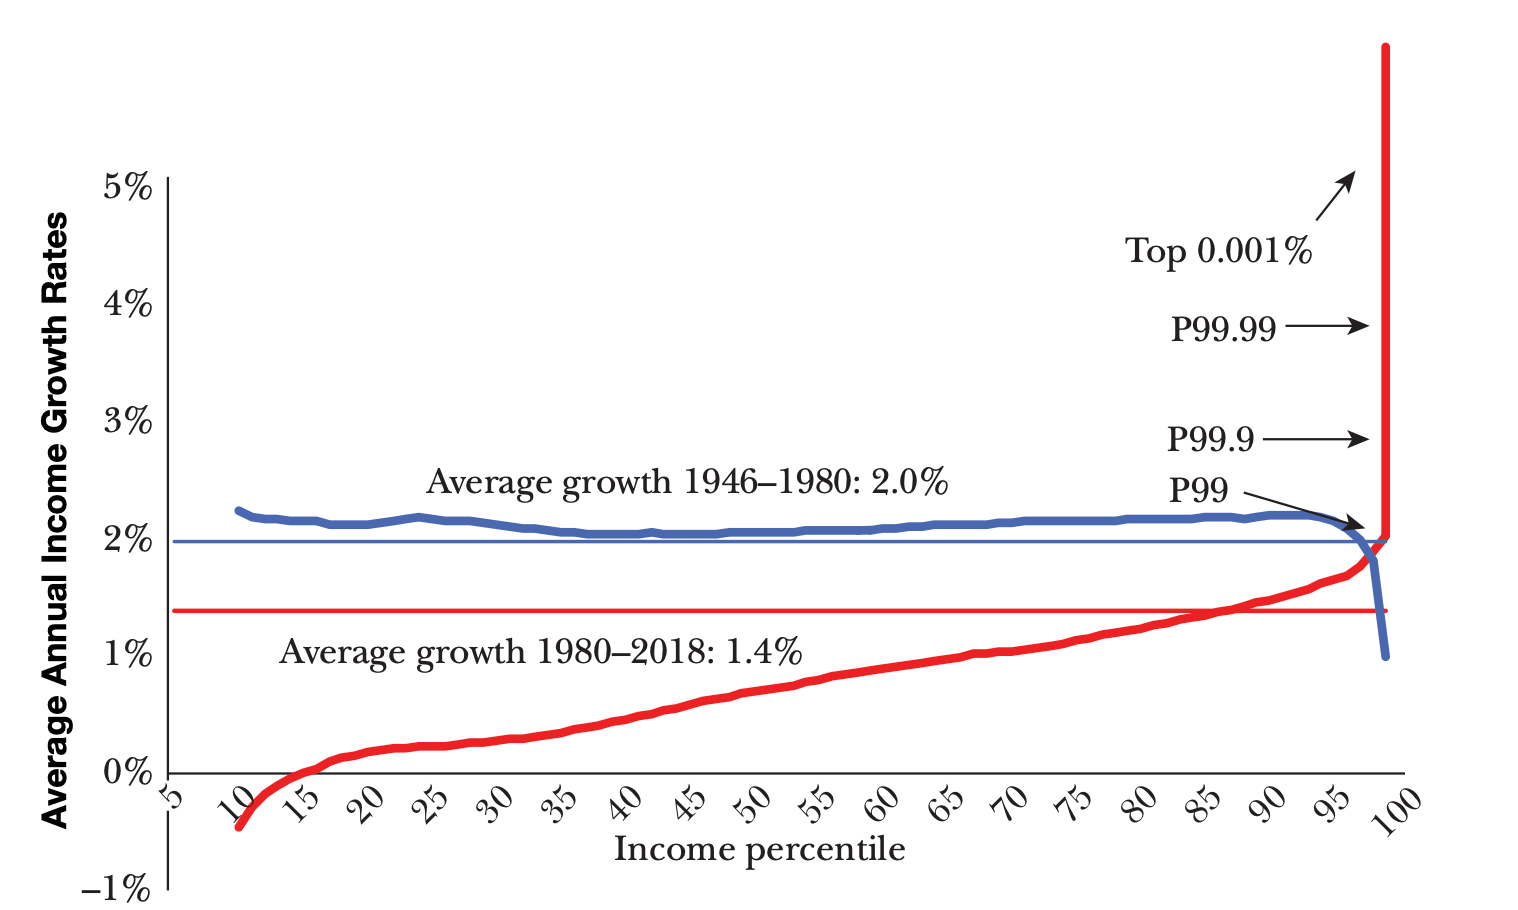
\includegraphics[width=0.8\textwidth]{images/bottom_stagnation_2.png}
    \end{center}
    \begin{center}
      Fact 3: Top 10\% share of income is U-Shaped in Anglophone countries, but L-shaped in Continental Europe and Japan. There is a large increase in inequality in many developing countries\\
      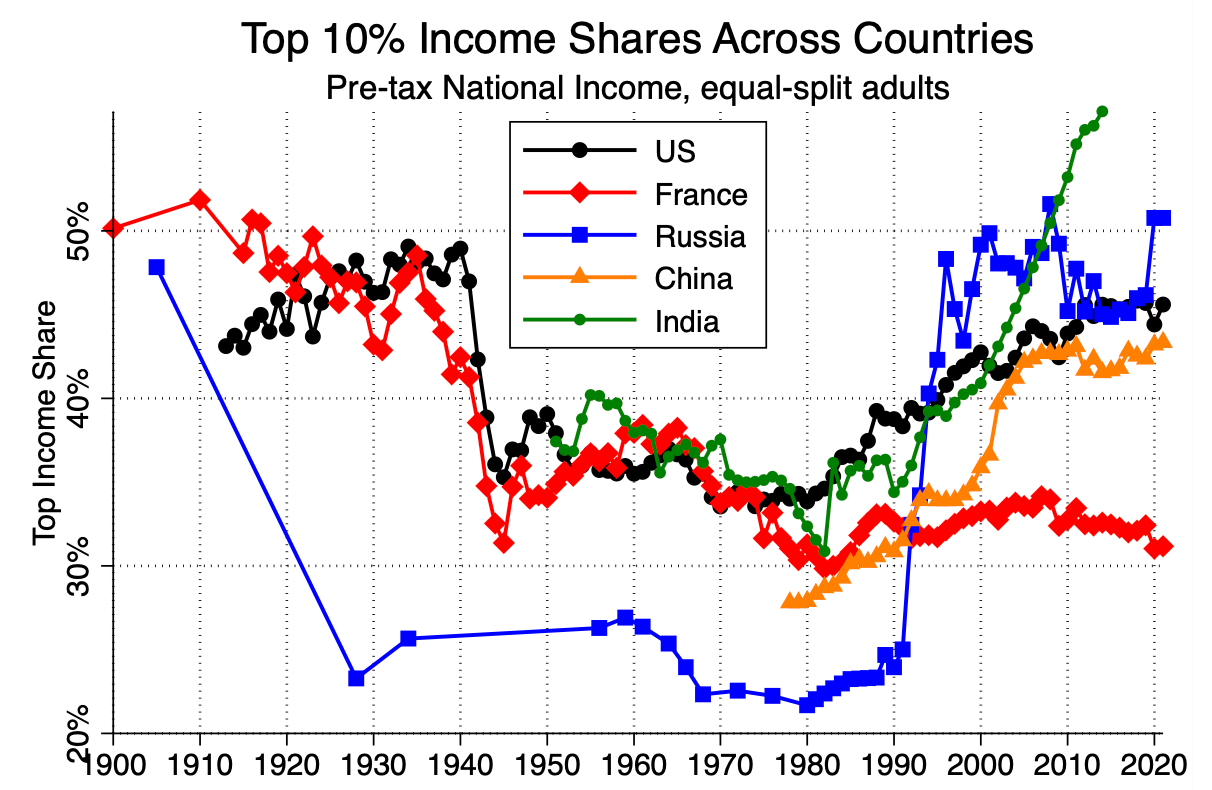
\includegraphics[width=0.8\textwidth]{images/country_inequality.png}
    \end{center}
  \end{problem}
  \begin{problem}{Measuring Poverty}
    We define the poverty rate as the fraction of a population with disposable income normalized by household size below the threshold $z^*$.
    \begin{itemize}
      \item Absolute Poverty: $z^*$ is fixed \textit{in real terms}. The World Bank uses a measure of \$2.15/person/day in 2017 dollars. There will not always be absolute poverty.
      \item Relative Poverty: $z^*$ is fixed \textit{relative to the median}. The European Union uses 60\% of median. There will always be relative poverty.
    \end{itemize}
    We can also measure poverty based on consumption $c$, not pre-tax market income.
    \begin{align*}
      c &= z - T(z) + B(z) + K(z) + E - s
    \end{align*}
    where
    \begin{itemize}
      \item $T(z)$ is income taxes and credits
      \item $B(z)$ is cash transfers
      \item $K(z)$ is in-kind government transfers
      \item $E$ is net private transfers
      \item $s$ is net savings
    \end{itemize}
    However, consumption is difficult to measure.
  \end{problem}
  \begin{problem}{How the US Measures Poverty}
    \begin{itemize}
      \item Definition developed in 1963 by Molly Orshansky at SSA as 3 times the amount required to buy a ``thrifty food plan''
      \item Based on annual \textit{family} \textbf{money income}
        \begin{align*}
          z_{m} &= z + B(z) + E
        \end{align*}
      \item Excludes taxes, tax credits, and in-kind transfers.
      \item Threshold adjusted annually using CPI.
    \end{itemize}
    Over time, the poverty rate has decreased from around 20\% in 1960 down to around 12\% in 2021.
  \end{problem}
  \begin{problem}{Redistribution Methods}
    The government taxes income and consumption and provides transfers:
    \begin{align*}
      y &= z - T(z) + B(z) + K(z)
    \end{align*}
    If inequality in $y$ is more than inequality in $z$, then the tax and transfer system is regressive --- if inequality in $y$ is less than in $z$, then the tax and transfer system is progressive.
    \begin{itemize}
      \item If $y = z(1-\tau)$, then the tax and transfer system is neutral.
      \item If $y = z(1-\tau) + R$, where $R$ is a universal transfer, then the tax and transfer system is progressive. Actual tax and transfer systems in rich countries work roughly like this.
    \end{itemize}
    Overall, the United States's tax and transfer scheme is progressive --- while the system's raw progressivity (in terms of effective tax rates) has declined, the level of redistribution has increased despite declining effective tax rates for the rich.
  \end{problem}
  \begin{problem}{Redistribution Motivations Activity}
    \begin{tcbraster}[raster columns = 1,colframe = black!75!white,colback=white]
      \tcbincludepdf{images/activity_8.pdf}
    \end{tcbraster}
  \end{problem}
  \begin{problem}{Tax Incidence}
    \textbf{Tax incidence} is the effect of tax policies on prices and the economic welfare of individuals. Incidence is analyzed at different levels:
    \begin{itemize}
      \item Producer vs. Consumer: effect of the tax on income/welfare of consumers vs. shareholders vs. producers of intermediate goods.
      \item Source of income: taxes on labor income vs. capital income vs. land income.
      \item Income level: progressivity of the labor income tax.
      \item Spatial/Regional: effect of a property tax increase on residents of one area vs. another area.
      \item Intergenerational: effect of the social security payroll tax on income/welfare of young vs. old.
    \end{itemize}
    Tax incidence is a \textbf{positive analysis}, we only analyze the impact of taxes.
  \end{problem}
  \begin{problem}{Key Results of Tax Incidence}
    \begin{description}
      \item[Key Result 1:] The statutory incidence of a tax is \textit{not} equal to the economic incidence of a tax. Taxes can shift relative prices.
        \begin{itemize}
          \item For example, liberals tend to favor increased capital income taxation because capital income is concentrated at the high end of the income distribution.
          \item However, if people save less because of the increased capital taxes, then capital stock goes down, and marginal product of \textit{labor} (i.e., wages) can go down due to reduced capital stock.
        \end{itemize}
      \item[Key Result 2:] Equilibrium is independent of who nominally pays the tax.\\

        We will focus on \textbf{partial equilibrium} in a \textbf{perfectly competitive} market.
        \begin{itemize}
          \item Assume that the government levies an excise tax $t$ on a good --- excise taxes are levied on a quantity (e.g., a \$1/pack tax on cigarettes). This is contrasted with \textit{ad valorem} taxes, which are on a particular fraction of prices (e.g., a 9\% sales tax).
          \item The supply function $S(p)$ depends on the producer price $p$, and the demand function $D(q)$ depends on the consumer price $q$.
          \item In equilibrium, $S(p) = D(q)$, and $t = q-p$.
          \item Therefore, with a producer tax, we have $S(q-t) = D(q)$, and for a consumer tax, we have $S(p) = D(p+t)$.
        \end{itemize}
      \item[Key Result 3:] The more inelastic factor bears more of the tax.
        \begin{align*}
          \frac{dp}{dt} &= \frac{\varepsilon_D}{\varepsilon_S - \varepsilon_D} \in [-1,0]\\
          \frac{dq}{dt} &= \frac{dp + dt}{dt}\\
                        &= \frac{\varepsilon_S}{\varepsilon_S - \varepsilon_D} \in [0,1]
        \end{align*}
        If $\varepsilon_D$ is close to $0$, then consumers bear more of the tax. Meanwhile, if $\varepsilon_S$ is close to $0$, then producers bear more of the tax.\\

        In the limiting cases, if $\varepsilon_D = -\infty$, then consumers bear $0\%$ of the tax, while if $\varepsilon_D = 0$, then consumers bear $100\%$ of the tax.
    \end{description}
  \end{problem}
  \begin{problem}{Tax Incidence in General Equilibrium}
    So far, we have focused on taxation in partial equilibrium (where we focus on the effect of the tax on one market in isolation).\\

    \textbf{General equilibrium} models consider the effects on related markets of a tax imposed on one market. For example, imposing a tax on cars may reduce demand for steel, which affects prices for other products beyond that of the car market.
  \end{problem}
  \begin{problem}{General Equilibrium Analysis: Berkeley Soda Tax}
    Consider the market for soda in Berkeley, California.
    \begin{itemize}
      \item Berkeley imposed a soda tax in 2015 of \$0.01 per ounce.
      \item The goal of the tax was to reduce soda consumption, and thereby improve health outcomes.
      \item If soda demand in Berkeley is inelastic, consumers bear more of the burden, but demand for soda \textit{in Berkeley} is likely to be elastic --- consumers consume less soda or buy soda in Oakland.
    \end{itemize}
    Consider the extreme case: perfectly elastic demand for soda.
    \begin{itemize}
      \item As a result, Berkeley soda sellers bear the full burden of the tax.
      \item However, soda sellers are made up of land, capital (buildings, kitchen equipment, etc.) and labor (cashiers, cooks, waitstaff, etc.)
      \item These two factors must bear the loss as a result of the tax --- incidence is ``shifted backward'' to land, capital, and labor.
    \end{itemize}
    \begin{description}
      \item[Short Run Incidence:]\hfill
        \begin{itemize}
          \item Assume that labor is perfectly elastic (workers can go to Oakland if they get paid less in Berkeley).
          \item However, given that restaurants/shops have fixed leases, we can also assume that capital is perfectly inelastic. Additionally, land in Berkeley is perfectly inelastic, seeing as you can't move land or make more land in Berkeley.
          \item Therefore, capital and land bear the tax in the short run.
        \end{itemize}
      \item[Long Run Incidence:]\hfill
        \begin{itemize}
          \item However, in the long run, capital is highly elastic --- restauranteurs can close, sell, and take their money to invest elsewhere, or sign a different lease.
          \item Therefore, in the long run, we assume that (physical) capital is perfectly elastic.
          \item So, we can assume that landowners are those that bear the incidence of the soda tax in the long run, assuming full elasticity of soda demand, labor, and capital are fully elastic.
        \end{itemize}
    \end{description}
    This is an idealized example --- in practice, soda demand, labor, and capital are not fully elastic, so incidence is shared in the long run.
  \end{problem}
  \begin{problem}{Federal vs. Total Tax Rates}
    The federal tax system is very progressive --- higher income and wealth individuals are taxed more than lower income and wealth individuals. However, state and local taxes are less progressive.\\

    Saez and Zucman (2019) found that most people across the income distribution pay around 25--30\%. Poorer individuals pay more in consumption and payroll taxes, while middle--high income individuals pay more in individual income taxes, and extremely wealthy individuals pay more of their income in corporate and property taxes.
  \end{problem}
  \begin{problem}{Tax Incidence Activity}
    \begin{tcbraster}[raster columns = 1,colframe = black!75!white,colback=white]
      \tcbincludepdf{images/activity_9.pdf}
    \end{tcbraster}
  \end{problem}
  \begin{problem}{Efficiency Costs of Taxation}
    Incidence is concerned with how taxes affect equilibrium prices and the \textit{distribution} of the proverbial economic pie.\\

    A second set of general questions is to understand how taxes affect the \textit{size} of the proverbial economic pie. Governments impose taxes to:
    \begin{itemize}
      \item Raise revenue to fund public goods and social insurance
      \item Redistribute income
    \end{itemize}
    However, raising tax revenue has an efficiency cost --- to generate \$1 of revenue, welfare of those taxes falls by more than \$1 due to behavior distortion.\\

    Deadweight Loss (DWL), or excess burden, is defined as the welfare loss created by a tax over and above the tax revenue generated by the tax.
  \end{problem}
  \begin{problem}{Insights from Deadweight Loss}
    Assuming no income effects and competitive production, we calculate the DWL of a tax by finding the area of the \textit{Harberger Triangle}:
    \begin{align*}
      \text{DWL} &= \frac{1}{2}(-dQ)(dt) \tag*{recall that $dQ$ is negative}\\
                 &= \frac{(\varepsilon_S)(-\varepsilon_D)}{2(\varepsilon_S - \varepsilon_D)}\cdot \frac{Q}{p} \cdot (dt)^2
    \end{align*}
    \begin{description}
      \item[Insight 1:] DWL increases with the absolute size of elasticities (i.e., it is more efficient to tax relatively inelastic goods).
      \item[Insight 2:] DWL increases with the \textit{square} of the tax rate (i.e., more efficient to have lower rates and broader bases than higher rates with smaller bases).
    \end{description}
  \end{problem}
  \begin{problem}{Optimal Commodity Taxation}
    Ramsey (1927) was asked Pigou to solve the following problem:
    \begin{itemize}
      \item Consider one consumer who consumes $K$ different goods.
      \item What are the tax rates $t_1,t_2,\dots,t_K$ on each good that raise a given amount of revenue while minimizing the welfare loss to the individual?
    \end{itemize}
    Obviously, uniform rates are not optimal if there are more elastic demands for certain goods.\\

    \textbf{Ramsey Rule:} the optimal tax rates are such that the marginal DWL for the last dollar of tax collected is the same across all goods:
    \begin{align*}
      \frac{M\text{DWL}_k}{MR_k} &= c, \tag*{for all $k = 1,2,\dots,K$}
    \end{align*}
    where $c$ is the marginal value of government revenue.
    \begin{description}
      \item[Implication:] Tax more the goods that have inelastic demand (and tax less the goods that have elastic demand)
      \item[Limitation:] Ramsey's result abstracts from redistribution and focuses solely on efficiency
    \end{description}
  \end{problem}
  \begin{problem}{Note on Income Effects}
    If we don't assume away income effects, the Harberger triangle \textit{overstates} DWL, since income effects do not create an efficiency cost.\\

    If there is a \$100 per person lump sum tax, consumers buy less and achieve lower welfare, but the DWL of the tax is zero because the amount the government would need to spend to arrive back at original welfare is \$100 --- the exact amount of revenue gained from the lump sum tax.
  \end{problem}
  \begin{problem}{Tax Salience}
    Standard economic models assume that individuals are fully aware of what they pay, but this is not necessarily so.\\

    Chetty, Looney, and Kroft (2009) test this assumption and develop a theory of taxation with inattentive consumers.
  \end{problem}
  \begin{problem}{Chetty et al. (2009) Empirical Strategy}
    \begin{description}
      \item[Randomized Field Experiment]\hfill
        \begin{itemize}
          \item In a treatment store, they display new price tags showing the levels of sales tax and total price on a subset of products.
          \item Researchers compare shopping behavior for treated products vs. control products in treated store, before and after new tags are implemented (DD estimator).
          \item They then repeat analysis in control stores as a \textit{placebo} DD estimator.
        \end{itemize}
      \item[Quasi-Experiment]\hfill
        \begin{itemize}
          \item Use variation in beer excise and sales taxes across states.
          \item Excise tax is salient because they're built into the posted price.
          \item Sales tax is not salient because it is not included in the posted price.
        \end{itemize}
    \end{description}
    \begin{description}
      \item[RFE Results:] Posting sales taxes reduces demand for particular goods by 7.6\%.
      \item[Quasi-Experiment Results:] Beer consumption is elastic to excise tax rates but not to sales tax rates.
    \end{description}
    Key result: tax salience matters --- if tax is not salient, then demand is less elastic, and consumers bear more of the tax burden.\\

    A number of empirical studies show that individuals are not fully informed and/or attentive; important consequences for policy.
  \end{problem}
  \begin{problem}{Commodity Taxation Activity}
    \begin{tcbraster}[raster columns = 1, sharp corners, colframe = black!75!white,colback=white]
      \tcbincludepdf{images/activity_10.pdf}
    \end{tcbraster}
  \end{problem}
  \begin{problem}{Taxation across Countries}
    As a share of GDP, OECD economies on average:
    \begin{itemize}
      \item Collect 34\% of GDP in tax revenue
      \item Spend 20\% of GDP on social transfers
    \end{itemize}
    Should governments mitigate inequality using transfers and taxes? If so, how?
  \end{problem}
  \begin{problem}{Transfers in the United States}
    \begin{itemize}
      \item Universal Transfers: public education, healthcare, social insurance (retirement, disability, unemployment)
      \item Means-tested transfers:
        \begin{itemize}
          \item In-Kind transfers: Medicaid, public housing, SNAP
          \item Cash transfers: TANF, Supplemental Security Income
        \end{itemize}
        Means-tested transfers tend to have high take-up costs, and (relatively) low utilization.
      \item Refundable Tax Credits: EITC; managed by the IRS, paid as lump-sum, low take-up costs and high utilization.
    \end{itemize}
  \end{problem}
  \begin{problem}{Types of Taxes}
    \begin{itemize}
      \item Consumption Taxes: sales taxes and excise taxes (value-added taxes in other countries)
      \item Payroll Taxes: taxes on labor earnings, funds Social Security and Medicare
      \item Individual Income Tax: taxes on a broader income base; includes labor income (wages), capital income (interest, dividends, and business income), and land income (rent, not including imputation from owner-occupancy)
      \item Corporate income tax: taxes on corporate profits net of reinvestment.
      \item Wealth taxes: taxes primarily on property (more common locally) and estates (e.g. inheritance)
    \end{itemize}
  \end{problem}
  \begin{problem}{Definition of Income}
    \begin{itemize}
      \item Income tax $T(z)$ is a function of annual household taxable income, $z$.
      \item $z$ is defined as \textbf{adjusted gross income} (AGI), net of standard or itemized deductions.
        \begin{itemize}
          \item AGI = Gross Income net of ``above-the-line'' deductions (healthcare premiums, pensions, etc.)
          \item AGI base is approximately 70\% of national income
          \item Standard Deduction is \$13850 for singles and \$27700 for couples in 2023
          \item Itemized deductions are taken in place of the standard deduction: state/local taxes (up to \$10K), interest on mortgages, or charitable giving are the most common itemized deduction.
        \end{itemize}
    \end{itemize}
  \end{problem}
  \begin{problem}{Marginal Tax Rates and Brackets}
    $T(z)$ is a continuous piecewise linear function with slope equal to MTR by taxable income bracket. $T'(z)$, which reflects the marginal tax rate, is a step function.
    \begin{center}
      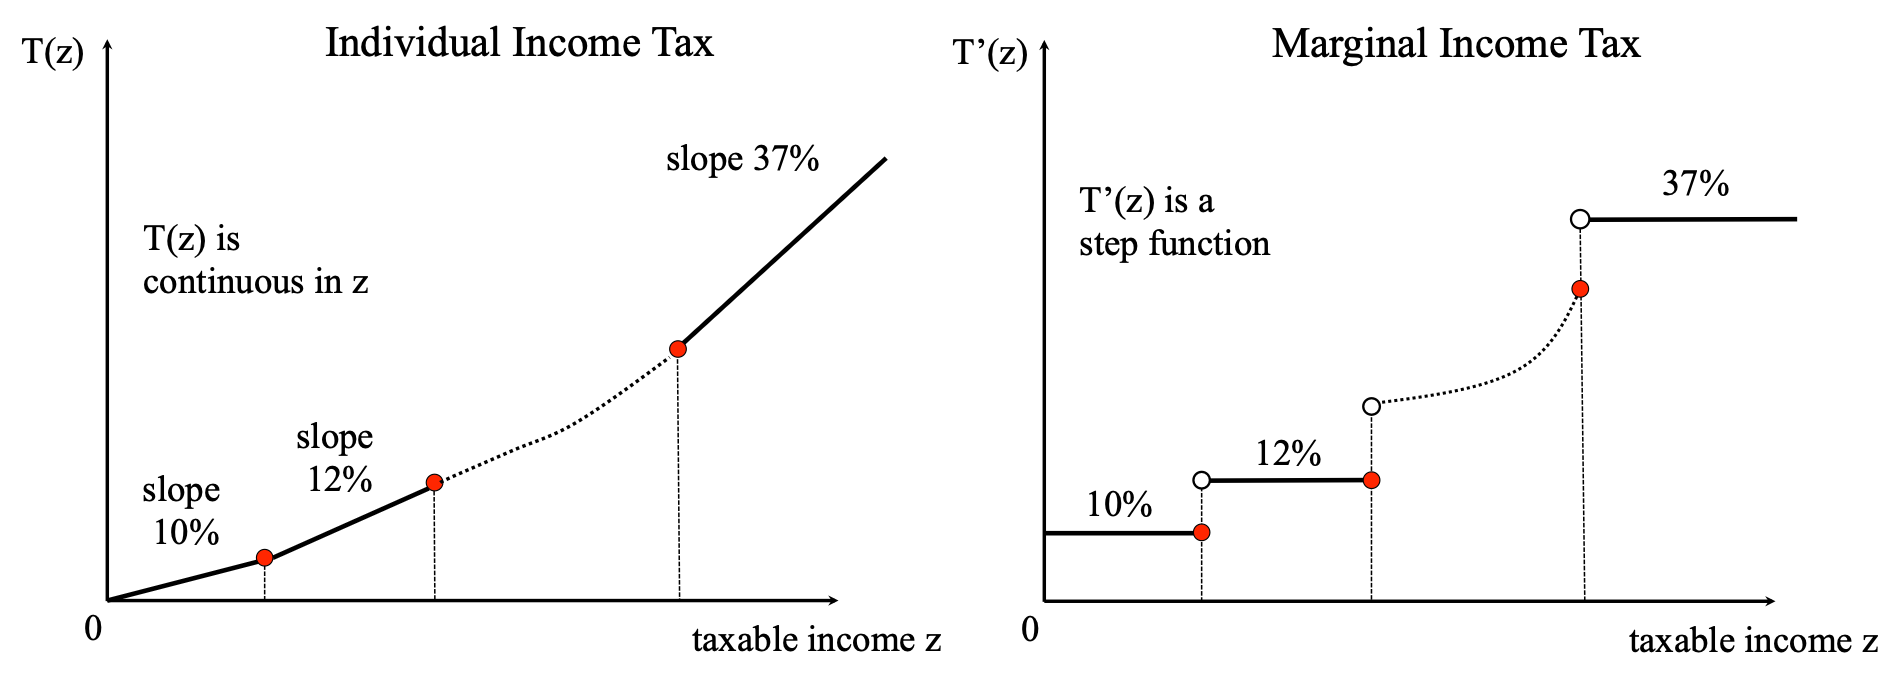
\includegraphics[width=0.8\textwidth]{images/MTRs.png}
    \end{center}
  \end{problem}
  \begin{problem}{Tax Credits}
    Tax credits are additional reductions in taxes above and beyond a deduction.
    \begin{itemize}
      \item Non-refundable credits (cannot reduce net tax burden below zero): foreign tax credits (offset taxes paid abroad), childcare expenses, residential energy efficient credits, etc.
      \item Refundable credits (can reduce net taxes below zero/act as a transfer): Child tax credit (\$2K per child, partially refundable), EITC (up to \$3.6K, \$5K, \$6.7K, based on family size)
    \end{itemize}
  \end{problem}
  \begin{problem}{Tax and Transfer Credits}
    \begin{itemize}
      \item Draw budget constraint $c = z - T(z)$ that integrates taxes and transfers
      \item Demogrant: $T(0)$, net transfer with zero earnings
      \item Marginal tax rate: $T'(z)$: individual keeps $1-T'(z)$ for every additional \$1 of earnings (intensive margin of labor supply)
      \item Break-even earnings point $z^{\ast}$: point where $T(z^{\ast}) = 0$
      \item Participation tax rate: $\tau_p = [T(z)-T(0)]/z$: individual keeps $1-\tau_p$ of earnings when moving from zero earnings to $z$ (extensive margin of labor supply) --- average slope of post-tax income
    \end{itemize}
  \end{problem}
  \begin{problem}{Optimal Income Taxation: No Behavioral Response}
    What is the optimal labor income tax function $T(z)$?\\

    Suppose everyone has the same concave utility function $u(c)$ over after-tax income $c = z - T(z)$, and there are two individuals with fixed incomes $z_1 < z_2$.\\

    We want to find $T(z)$ that maximizes Utilitarian SWF:
    \begin{align*}
      f(z_1,z_2) &= u(z_1-T(z_1)) + u(z_2 - T(z_2))\\
      0 &= T(z_1) + T(z_2)\\
      \shortintertext{Both of which imply}
      z_1 - T(z_1) &= z_2 - T(z_2)
    \end{align*}
    This implies 100\% redistribution --- perfect equalization of after-tax income --- mathematically equivalent to full insurance with risk aversion and no moral hazard. However, this is unrealistic:
    \begin{itemize}
      \item 100\% redistribution would remove all incentive to work, so the assumption that $z$ is fixed is unrealistic.
      \item With utilitarianism, behavioral responses are the only factor preventing complete redistribution. However, not everyone is a utilitarian, and citizens' views on fairness bound the ability of the government to redistribute.
    \end{itemize}
    \rule{\textwidth}{0.4pt}
    \vspace{4pt}
    Maybe we can use the Second Welfare Theorem?
    \begin{itemize}
      \item Second Welfare Theorem: Any Pareto efficient outcome can be reached via a suitable set of lump sum taxes (based on intrinsic earning ability), then letting markets work freely
      \item There is no conflict between efficiency and equity, right?
    \end{itemize}
    However, governments must base taxes and transfers based on actual earnings, rather than intrinsic earnings ability --- there is a real conflict between efficiency and equity.
  \end{problem}
  \begin{problem}{Tax Effect Activity}
    \begin{tcbraster}[raster columns = 2, sharp corners, colframe = black!75!white,colback=white]
      \tcbincludepdf{images/activity_11.pdf}
    \end{tcbraster}
  \end{problem}
  \begin{problem}{Optimal Labor Income Taxation}
    Assume individuals pay a linear tax rate $\tau$ on earnings $z$ and receive a fixed universal transfer $R$. There are $N$ individuals, with each person $i$ choosing their utility-maximizing labor supply $l_i$ by maximizing
    \begin{align*}
      u^i(c_i,l_i) = u^i\left((1-\tau)w_il_i + R, l_i\right)
    \end{align*}
    The government budget is
    \begin{align*}
      R &= \tau \cdot Z\\
      Z &= \sum_{i}z_i/N,
    \end{align*}
    meaning average tax revenue is $R(\tau) = \tau\cdot Z(1-\tau)$. Therefore, at $\tau = 0$, no tax revenue (meaning no one works), and at $\tau = 1$, no one works due to no incentive to do so.
    \begin{center}
      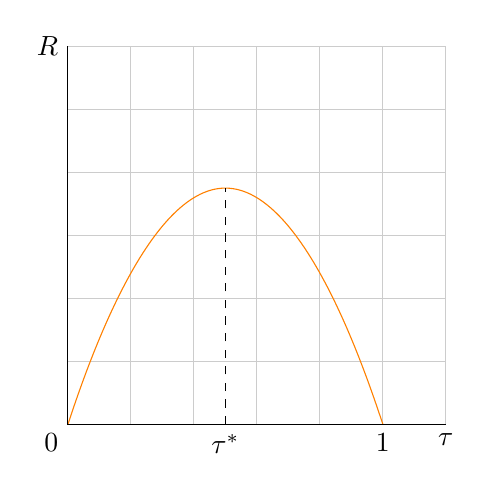
\begin{tikzpicture}[scale=4]
        \draw[black!20!white,step=0.2] (0,0) grid (1.2,1.2);
        \draw[color = orange] (0,0) parabola[parabola height=0.75cm] +(1,0);
        \node[anchor = east] at (0,1.2) {$R$};
        \node[anchor = north] at (1.2,0) {$\tau$};
        \draw[dashed] (0.5,0) -- (0.5,0.75);
        \node[anchor = north] at (0.5,0) {$\tau^{\ast}$};
        \node[anchor = north east] at (0,0) {$0$};
        \node[anchor = north] at (1,0) {$1$};
        \draw (0,1.2) -- (0,0) -- (1.2,0);
      \end{tikzpicture}
    \end{center}
    Known as the Laffer curve, although the idea dates back to Dupuit (1844), revenue is maximized in this simplistic model at $\tau = \tau^{\ast}$. It is inefficient to have $\tau > \tau^{\ast}$. Under the Rawlsian framework, we want to maximize $R$, meaning that $\tau = \tau^{\ast}$.\\

    To determine $\tau^{\ast}$, we consider the effect of an increase in the tax rate by $d\tau > 0$.
    \begin{itemize}
      \item Mechanical Effect: increases average tax revenue (by increasing tax rates) --- $dM = Z\cdot d\tau > 0$
      \item Behavioral Effect: reduces average tax revenue (by reducing labor supply) --- $dB = \tau \cdot dZ < 0$
    \end{itemize}
    At the optimum, $dM + dB = 0$ (i.e., maximizing tax rates).
    \begin{align*}
      \tau^{\ast} &= \frac{1}{1+e}\\
      \shortintertext{where}
      e &= \frac{1-\tau}{Z}\frac{dZ}{d(1-\tau)}\\
      \shortintertext{is the elasticity of average income with respect to the net-of-tax rate. There are different estimates of $e$, but $e = 0.25$ implies that $\tau^{\ast} = 80\%$.}
    \end{align*}
    Under a utilitarian framework, we want to maximize
    \begin{align*}
      SWF &= \sum_{i}u^i(c_i,l_i)\\
          &= \sum_{i}u^i\left((1-\tau)w_il_i + \tau\cdot Z(1-\tau), l_i\right)
    \end{align*}
    taking into account that labor supply responds to tax policy. In this scenario, the optimal linear income tax rate is
    \begin{align*}
      \tau &= \frac{1-\overline{g}}{1-\overline{g} + e}
    \end{align*}
    where $\overline{g} \in [0,1]$ measures the degree of pre-tax earnings equality.\\

    This formula captures the equity-efficiency tradeoff:
    \begin{itemize}
      \item $\tau$ is decreasing in behavioral elasticity $e$
      \item $\tau$ is decreasing in pre-tax earnings equality $\overline{g}$
    \end{itemize}
    The formula is very general and applies if:
    \begin{itemize}
      \item People respond to taxation by dropping out of the labor force instead of adjusting hours.
      \item People choose education based on tax rate.
      \item Earnings are generated by a combination of ability and luck.
    \end{itemize}
  \end{problem}
  \begin{problem}{Optimal \textit{Top} Income Tax Rate}
    Consider a constant marginal tax rate $\tau$ above fixed $z^{\ast}$. Denote $z_m$ to be the \textit{mean} income of top bracket earners. Let elasticity of $z_m$ with respect to net-of-tax rate be
    \begin{align*}
      e = \frac{1-\tau}{z_m}\cdot \frac{dz_m}{d(1-\tau)}
    \end{align*}
    Assume a small $d\tau > 0$ tax increase. Then, we have
    \begin{itemize}
      \item Mechanical Effect: $dM = d\tau \cdot (z_m - z^{\ast})$
      \item Behavioral Effect: $dB = \tau dz_m$
    \end{itemize}
    We find that the optimal top tax rate is
    \begin{align*}
      \tau &= \frac{1}{1+ae}\\
      a &= \frac{z_m}{z_m-z^{\ast}}
    \end{align*}
    where $a$ denotes the Pareto coefficient --- i.e., the average income of people who make above the income threshold. In the United States, $a \approx 1.5$ --- i.e., $z_m = 3z^{\ast}$.\\

    Estimating $e$ is very hard:
    \begin{itemize}
      \item If $e = 0.25$, then $\tau^{\ast}_m = 73\%$
      \item If $e = 0.5$, then $\tau^{\ast}_m = 57\%$
    \end{itemize}
  \end{problem}
  \begin{problem}{Optimal Labor Income Taxation}
    \begin{tcbraster}[raster columns = 2, sharp corners, colframe = black!75!white,colback=white]
      \tcbincludepdf{images/activity_12.pdf}
    \end{tcbraster}
  \end{problem}
  \begin{problem}{Optimal Transfers}
    What is the optimal structure of a transfer program? The answer depends on:
    \begin{enumerate}[(1)]
      \item how people respond to the tax/transfer policy:
        \begin{itemize}
          \item On the intensive margin (\textit{how much} to work)
          \item On the extensive margin (\textit{whether or not} to work)
        \end{itemize}
      \item how society weights the welfare of low income people relative to the average person
    \end{enumerate}
  \end{problem}
  \begin{problem}{Intensive Margin Response}
    Suppose that individuals respond to taxes only on the intensive margin, and society cares more about people with zero earnings.\\

    In this scenario, the optimal transfer takes the form of a ``negative income tax.''
    \begin{description}
      \item[Lump-Sum Grant:] $T(0) > 0$ for zero earners.
      \item[Marginal Tax Rates:] $T'(z)$ at the bottom to quickly phase out the grant. ($T'(z) \approx 80\%$)
    \end{description}
    The intuition:
    \begin{itemize}
      \item Targeting transfers to the most needy (zero earners)
      \item Earnings at the bottom are low $\Rightarrow$ intensive labor supply response from high marginal tax rate does not generate large tax revenue loss
    \end{itemize}
  \end{problem}
  \begin{problem}{Extensive Margin Response}
    Suppose that individuals respond to taxes only on the extensive margin, and society cares about low-income \textit{workers}.\\

    Then, the optimal transfer at the bottom subsidizes work with a \textit{negative marginal tax rate}, $T'(z) < 0$, meaning low-income workers get a bigger transfer than non-workers.
    \begin{itemize}
      \item Targets transfer to a deserving group.
      \item Incentivizes people to enter (or not drop out of) labor force.
    \end{itemize}
  \end{problem}
  \begin{problem}{Transfers In Practice}
    In practice, both intensive and extensive margins exist --- for low income people, extensive margin response is greater than intensive margin response.
    \begin{itemize}
      \item Optimal to have initially low or negative phase phase-out rates with higher phase-outs further up the income distribution.
      \item Structure matches trend in OECD countries to expand in-work benefits and lower MTRs for low income earners.
    \end{itemize}
  \end{problem}
  \begin{problem}{Universal Basic Income}
    \begin{itemize}
      \item All receive an unconditional sum of money regardless of how much they earn.
      \item Basic Income: give $R$ to all, tax all earnings $z$ at MTR $\tau$
      \item Basic income funded by labor taxes is economically equivalent to means-tested transfer phased out with earnings.
    \end{itemize}
    Benefits of UBI: less stigmatized than means-tested transfer, more widely accepted.\\

    Costs of UBI: higher nominal taxes (which are politically unpopular).
  \end{problem}
  \begin{problem}{In-Kind Transfers}
    Many rich-countries provide ``in-kind'' universal basic incomes in the form of healthcare and public education, but also many means-tested transfers are in-kind (healthcare, education assistance, housing, SNAP, etc.).
    \begin{description}
      \item[Individual Perspective:] Cash transfer is preferable to in-kind benefit.
      \item[Social Justifications:]
        \begin{itemize}
          \item Commodity Egalitarianism: some goods (education health, shelter, food) seen as \textit{rights} and ought to be provided to all
          \item Paternalism: society imposes its preferences on recipients
          \item Behavioral Mistakes: Recipients do not make choices in their best interest (self-control, myopia, inattention, etc.)
        \end{itemize}
    \end{description}
  \end{problem}
  \begin{problem}{Taxing Families}
    Two important questions in taxing families:
    \begin{itemize}
      \item Couples: optimal taxation of couples vs. singles.
      \item Children: what should be the net transfer to family with children?
    \end{itemize}
    There are three desirable properties in the question of taxation of families:
    \begin{enumerate}[(1)]
      \item based on family income --- families with equal incomes pay equal taxes
      \item marriage neutrality --- no higher/lower taxes when two single individuals marry
      \item progressive --- higher incomes pay a larger fraction of their income in taxes
    \end{enumerate}
    It is impossible to have a tax system that satisfies all $3$ conditions simultaneously, because the first two conditions imply
    \begin{align*}
      T(z_1 + z_2)&= T(z_1) + T(z_2),
    \end{align*}
    or a linear, non-progressive tax rate.\\

    There are two systems for taxing couples:
    \begin{itemize}
      \item Individual system: marriage neutral, can be progressive, but taxes someone married to a rich spouse the same as someone married to a spouse with no income.
      \item Family system: desirable from welfare perspective if couples share their incomes, but with progressive tax brackets, not marriage neutral.
    \end{itemize}
    In actuality, most countries use the individual system; only the US, Ireland, and Norway have a pure family tax system.
    \begin{itemize}
      \item If marriage responds strongly to tax penalty/subsidy, it's better to move toward the individual system. This is particularly important when cohabitation is a close substitute for marriage.
      \item If the labor supply of secondary earners is more elastic than the primary earner, it means secondary earners should be taxed less, achievable with individual taxes.
      \item However, the labor supply elasticity differential between primary and secondary earners is decreasing as gender earnings gap decreases.
    \end{itemize}
  \end{problem}
  \begin{problem}{Child Benefits}
    Most tax/transfer systems offer tax reductions for children.
    \begin{itemize}
      \item For a given family income, children reduce normalized family income $\Rightarrow$ children increase the marginal utility of consumption $\Rightarrow$ transfer for children should be positive.
      \item Two thoughts on the size of $T_{\text{kid}}(z)$:
        \begin{itemize}
          \item Not increase with income: lower income families need child transfers most
          \item Should increase with income: rich people work more and have higher childcare costs
        \end{itemize}
      \item In practice, $T_{\text{kid}}(z)$ is fairly constant with $z$. Europe has more generous pre-kindergarten childcare benefits, while the US has more generous cash tax credits.
    \end{itemize}
    In 2021, ARP expanded child tax credit, increasing its value, making it fully refundable, and paid out monthly.
    \begin{itemize}
      \item Child poverty rate fell by 46\% in 2021 to record low.
      \item However, spiked in 2022 as expanded CTC ended.
    \end{itemize}
  \end{problem}
  \begin{problem}{Responses to Labor Income Taxation}
    Labor supply responses to taxation are very important for understanding income tax policy (including efficiency costs and optimal tax formulas). The labor supply responds along many dimensions:
    \begin{enumerate}[(a)]
      \item Intensive margin: hours of work, effort, occupational choice, education
      \item Extensive margin: entry decisions in the labor market
      \item Reported earnings: tax avoidance (legally minimizing burden) and tax evasion (illegally underreporting)
      \item Time horizon: short-run effects of all these vs. long-run effects.
    \end{enumerate}
  \end{problem}
  \begin{problem}{Early Empirical Methods}
    Many studies used regression analyses to estimate total elasticity of labor supply with respect to net-of-tax wage:
    \begin{align*}
      e &= \frac{\%\Delta l}{\%\Delta(1-\tau)w}.
    \end{align*}
    The total effect can be decomposed into the sum of substitution effect and income effect.
    \begin{center}
      \begin{tabular}{c|c|c|c|}
        & Total Elasticity & Substitution Effect & Income Effect\\
        \cline{2-4}
        Male Workers (Primary Earners) & $0$ & $0.1$ & $-0.1$\\
        Female Workers (Secondary Earners) & $\sim 0.5$ & $0.5$ & $0$
      \end{tabular}
    \end{center}
    However, the cross-sectional regression approach has an identification problem; to resolve, we might exogenously increase the tax rate, but it's very costly to implement such true experiments.\\

    Modern studies use tax changes as quasi-experiments and DD estimators.\\

    In 2003, Germany made secondary jobs paying under 400 euros/month tax free, amounting to a 20--60\% subsidy on secondary job earnings; they found a large increase in second jobs without offsetting, meaning people did work more.\\

    In the United States, a 1993 law greatly expanded the Earned Income Tax Credit (EITC), and there was a large increase in labor force participation among single mothers after the reform. However, there were confounders:
    \begin{itemize}
      \item Traditional cash welfare was cut during the same period of time
      \item During the period of time examined, unemployment reduced substantially.
      \item Also during the same period of time, states were experimenting with different types of social welfare programs.
    \end{itemize}
  \end{problem}
  \begin{problem}{Theoretical Behavioral Responses to EITC}
    \begin{center}
      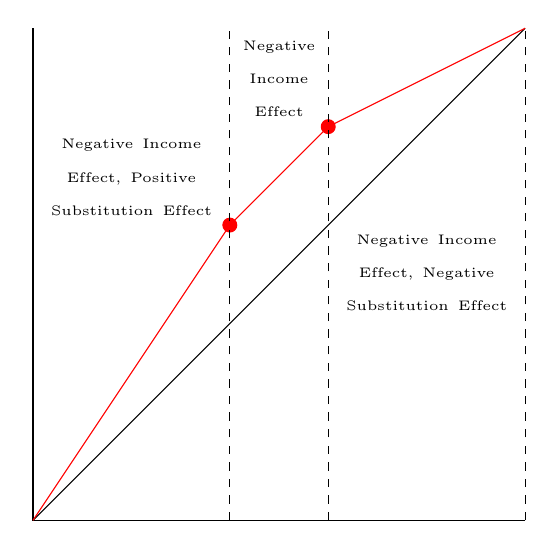
\begin{tikzpicture}[scale=1.25]
        \draw (0,5) -- (0,0) -- (5,0);
        \draw (0,0) -- (5,5);
        \draw[red] (0,0) -- (2,3) -- (3,4) -- (5,5);
        \filldraw[red] (2,3) circle (2pt)
                      (3,4) circle (2pt);
                      (5,5) circle (2pt);
        \draw[dashed] (2,0) -- (2,5);
        \draw[dashed] (3,0) -- (3,5);
        \draw[dashed] (5,0) -- (5,5);
        \node[align = center, anchor= south,text width=2.4cm] at (1,3){\tiny Negative Income Effect, Positive Substitution Effect};
        \node[align = center, anchor = south east, text width=1cm] at (3,4){\tiny Negative Income Effect};
        \node[align = center, anchor = north, text width = 2.4cm] at (4,3) {\tiny Negative Income Effect, Negative Substitution Effect};
      \end{tikzpicture}
    \end{center}
    \begin{itemize}
      \item Extensive Margin: Reducing participation tax rate $\Rightarrow$ positive effect on participation.
      \item Intensive margin: Earnings conditional on working can increase or decrease depending on segment of budget constraint.
    \end{itemize}
    Theoretically, we should see bunching close to the kink point where the tax rate increases, which is what Saez (2010) found.
    \begin{itemize}
      \item There is evidence of response along the extensive margin.
      \item Little evidence of response along the intensive margin, except for self-employed people.
      \item Together, this evidence implies that the optimal transfer looks like the EITC.
    \end{itemize}
  \end{problem}
  \begin{problem}{Sources of Deadweight Loss}
    Behavioral response to tax changes comes not only from adjusting labor supply hours, but also from:
    \begin{itemize}
      \item Other labor supply changes (such as effort, occupational choice, etc.)
      \item Tax avoidance.
      \item Ta evasion.
    \end{itemize}
    Modern public economics literature focuses on the elasticity of average reported taxable income (ETI).
    \begin{align*}
      e &= \frac{1-\tau}{z}\frac{\partial z}{\partial(1-\tau)}
    \end{align*}
    \begin{itemize}
      \item The optimal income tax formulas are in terms of $e$.
      \item Reported taxable income is precisely measured in tax return data
      \item Elasticity depends on features of the tax system (such as deductions, enforcement, tax base, etc.)
    \end{itemize}
    Piketty, Saez, and Stantcheva (2014) estimated $e$ via quasi-experiments from tax changes that affect similar populations differently.
    \begin{itemize}
      \item They found a clear correlation between top incomes and top income tax rates ($e\approx 0.5$ to $0.6$).
      \item There is a much lower elasticity below the top incomes ($e\approx 0.1$ to $0.2$).
      \item Top income shares sometimes do not respond to large tax rate cuts, suggesting that context (such as opportunity to respond to, avoid, or evade taxes).
    \end{itemize}
    There is a strong, but not perfect correlation between change in top marginal tax rates and change in share of top 1\% of (reported) income.
  \end{problem}
  \begin{problem}{Wealth and Taxes on Savings}
    Private wealth in the United States is approximately 6 times national income (originally was around 4 times national income, but increased dramatically since 1970).\\

    Much of wealth is a mixture of pensions and houses.
    \begin{itemize}
      \item Total wealth reflects both capital stock accumulated through savings and pure price effects.
      \item Houses can increase in value due to improvements or through local price increases (without an increase in commensurate capital stock).
      \item Increased monopoly power (such as patent ownership) makes a business more valuable, but reduces consumer utility.
      \item Recent increases in US private wealth is mostly due to price effects.
    \end{itemize}
    \begin{center}
      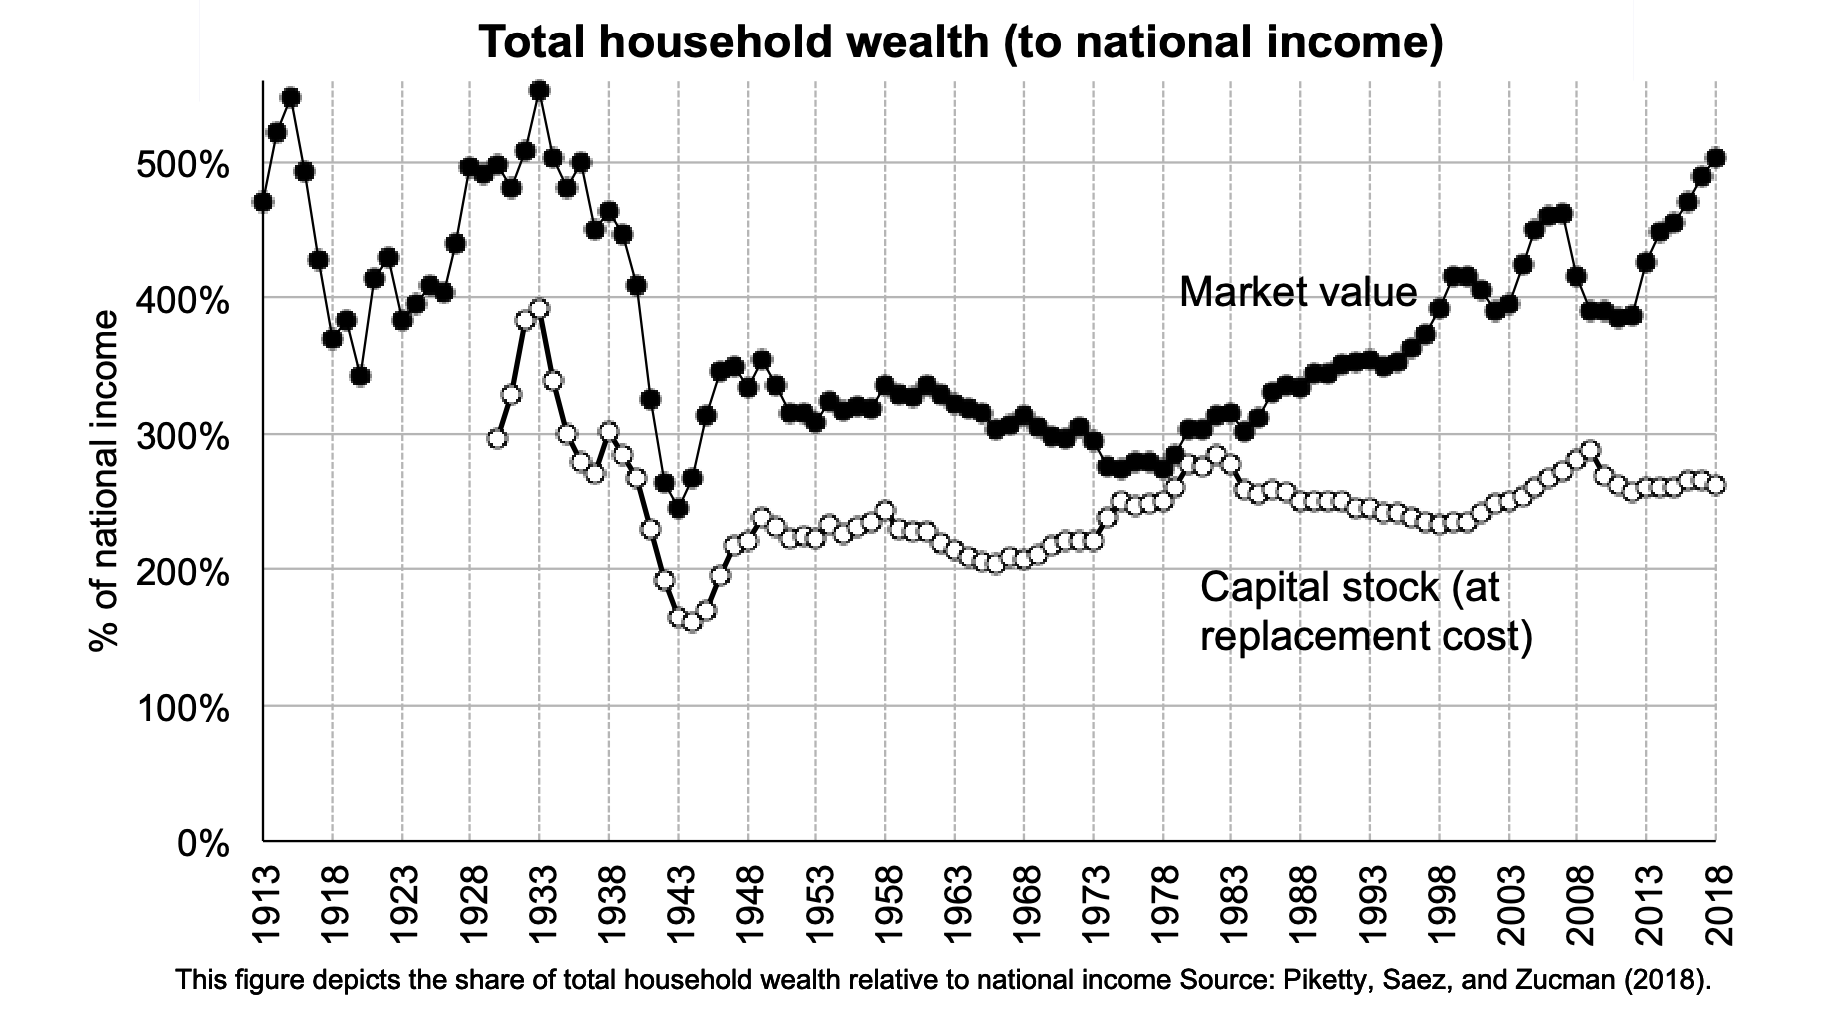
\includegraphics[width=10cm]{images/wealth_increase.png}
    \end{center}
    Wealth in the United States is distributed very unevenly --- average net worth for White Americans is about \$1M, while average net worth for Black Americans is around \$140,000. Net worth isn't accounted for by educational differences or debts, and even by income differences.\\

    However, this wealth gap is likely the long-run effect of historic racism (i.e., zoning laws, homeownership subsidies, etc.).\\

    The share of wealth for the top 0.1\% has grown substantially since the mid-1970s; additionally, as of 2021, 75\% of wealth is held by the top 10\% of wealth holders.\\

    People tend to underestimate wealth inequality (in part because incomes are distributed more equally than wealth).
  \end{problem}
  \begin{problem}{Modeling Wealth Accumulation}
    \begin{align*}
      W_{t} &= W_{t-1} + r_{t}W_{t-1} + E_t - C_t + I_t
    \end{align*}
    \begin{itemize}
      \item $W_t$: Wealth at period $t$
      \item $r_tW_{t-1}$: Capital income from period $t-1$ capital stock
      \item $E_t$: labor market earnings net of taxes
      \item $C_t$: consumption
      \item $I_t$: net inheritances
    \end{itemize}
    There are two types of wealth:
    \begin{itemize}
      \item Life-cycle wealth: $E_t-C_t$ is wealth from savings earlier in life
      \item Inherited wealth: $I_t$ is wealth from inheritances received
    \end{itemize}
    Distinction matters for taxation because individuals are responsible for life-cycle wealth but not inherited wealth.\\

    Inherited wealth as a proportion of total wealth has been increasing since the 1980s.\\

    Thomas Piketty, in \textit{Capital in the 21st Century}, saw that since return on wealth is higher than the rate of economic growth ($r > g$), wealth concentration and inherited wealth are increasing.
  \end{problem}
  \begin{problem}{Capital Taxation: Efficiency and Equity Concerns}
    Because wealth and capital income are more unequally distributed than labor income, equity concerns suggest it should be taxed more than labor
    \begin{itemize}
      \item Capital income taxation reduces $r$ to $r(1-\tau_k)$
    \end{itemize}
    However, capital accumulation correlates strongly with growth, and capital accumulation may be sensitive to the net-of-tax return, meaning that efficiency cost of capital taxation may be high.
  \end{problem}
  \begin{problem}{Capital Taxation in the United States}
    Individual income taxation in the United States taxes many forms of capital income:
    \begin{itemize}
      \item Interest earned from savings is taxed as ordinary income.
      \item Imputed rent from owner-occupancy and returns on deferred compensation are exempt.
      \item Realized capital gains and dividends receive preferential treatment (to lower double taxation of corporate profits)
      \item Capital gains on owner-occupied housing are exempt up to \$500K.
    \end{itemize}
    The estate tax is a 40\% federal tax on $I$ above \$13M/person.\\

    Property taxes on real estate amount to about 0.5\% of market value on average.\\

    Corporate taxes are at a nominal rate of 21\%, but the effective tax rate is lower.
  \end{problem}
  \begin{problem}{Modeling Taxes on Savings}
    Consider capital income tax $\tau_k$ on savings $s$ in a 2-period model with fixed earnings $w$ in period 1.\\

    Then, $c_1 + s = w$, and $c_2 = (1+r(1-\tau_k))s$, which gives
    \begin{align*}
      \max_{c_1,c_2}\left(u(c_1) + \delta u(c_2)\right)
    \end{align*}
    subject to
    \begin{align*}
      c_1 + \frac{c_2}{1 + r(1-\tau_k)} =w
    \end{align*}
    \begin{center}
      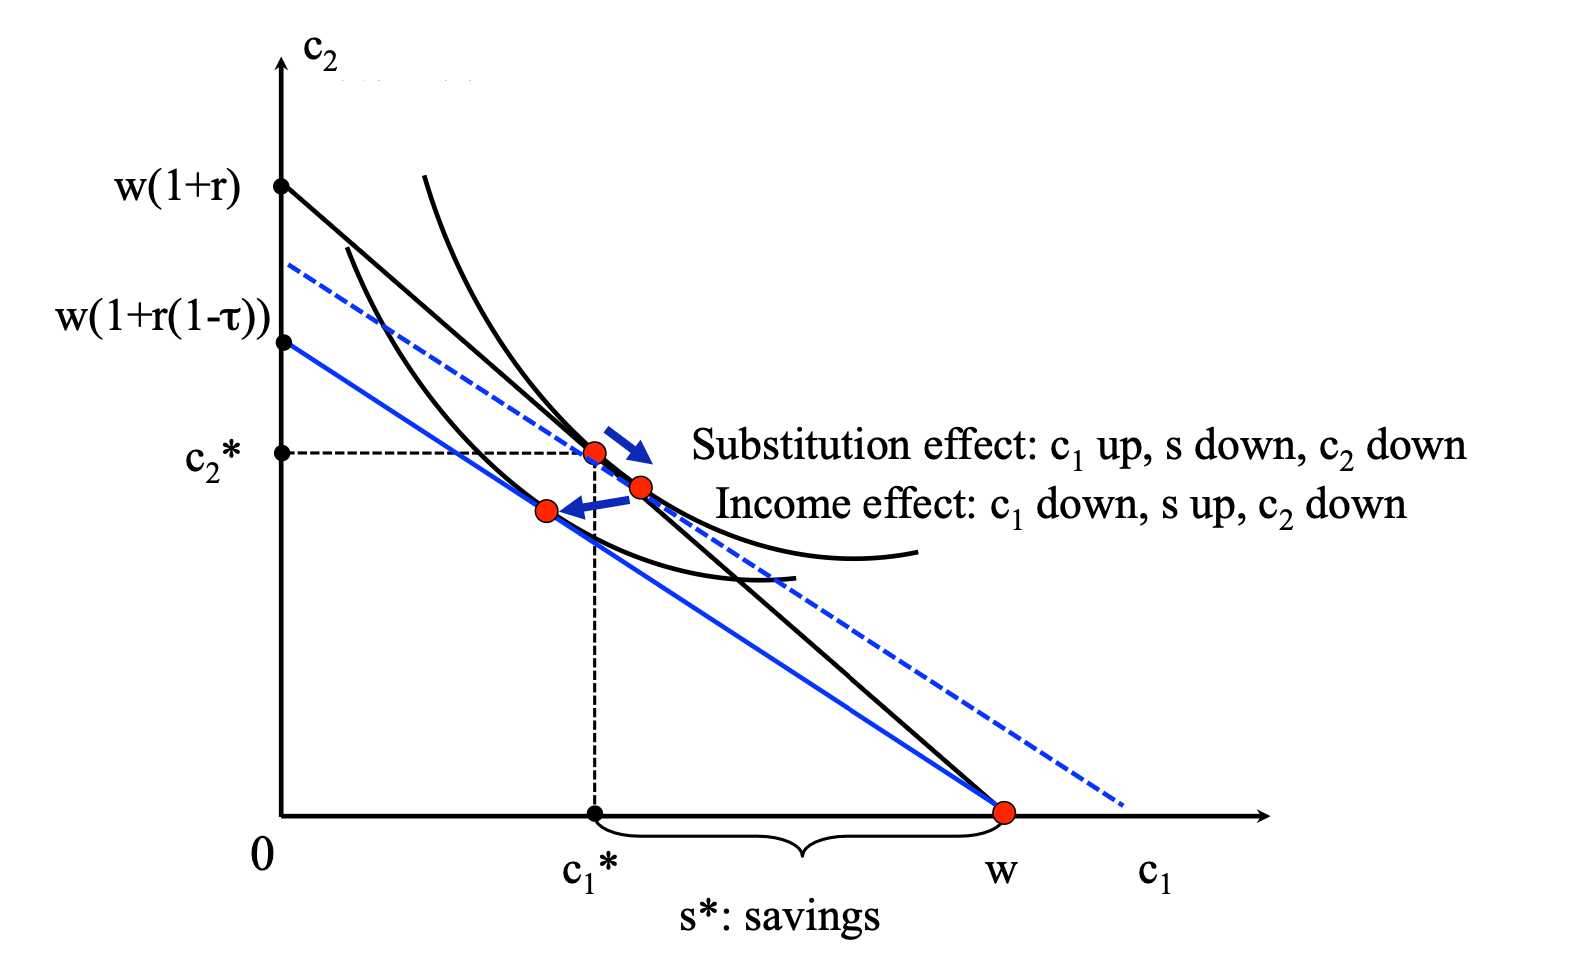
\includegraphics[width=10cm]{images/two_period_savings_tax.png}
    \end{center}
  \end{problem}
  \begin{problem}{Fundamental Tax Reform}
    Some advocate shifting to a consumption tax. To see how this compares to a current system, consider a simple intertemporal budget constraint with labor supply $l$.
    \begin{itemize}
      \item Consumption tax $t_c$:
        \begin{align*}
          (1+t_c)\left(c_1 + \frac{c_2}{1+r}\right) &\leq wl
        \end{align*}
      \item Consumption tax is equivalent to taxing only labor earnings at a rate $\tau_l$ if $1 + t_c = \frac{1}{1-\tau_l}$
        \begin{align*}
          c_1 + \frac{c_2}{1+r} &\leq (1-\tau_l)wl
        \end{align*}
      \item Both taxes only distort labor supply and not savings.
    \end{itemize}
    \begin{description}
      \item[Efficiency:] Moving to a consumption tax would eliminate the current savings distortion of the US tax system.
      \item[Transition:]\hfill
        \begin{itemize}
          \item Double taxation of transition generation.
          \item Generates one-time wealth tax
        \end{itemize}
      \item[Equity:] Actual consumption taxes tend to be regressive while actual income taxes are generally progressive.
    \end{description}
  \end{problem}
  \begin{problem}{Taxes on Wealth}
    In the life-cycle model, we suppose that the government can use a nonlinear labor income tax $T(wl)$ and a linear capital income tax $\tau_k$. We want to maximize $u(c_1) - h(l) + \delta u(c_2)$, subject to
    \begin{align*}
      c_1 + \frac{c_2}{1 + r(1-\tau_k)} &= wl - T(wl)
    \end{align*}
    \begin{description}
      \item[Atkinson-Stiglitz Theorem:] The optimal tax $\tau_K$ on capital income should be zero --- taxes on labor are sufficient.
        \begin{itemize}
          \item In the life-cycle model, inequality in lifetime resources is due solely to differences in earnings ability --- inequality can thus be addressed with labor income taxation.
          \item However, the theorem relies on many simplifications --- timing of income, preferences, patience, etc.
        \end{itemize}
    \end{description}
    There are other sources of capital income inequality:
    \begin{itemize}
      \item If high-wage individuals are able to invest in higher return assets, then taxing capital income is a way to mitigate such inequality.
      \item Differential tax treatment between capital and labor can induce tax avoidance.
      \item Inheritances.
    \end{itemize}
  \end{problem}
  \begin{problem}{Estate Tax and Optimal Inheritance Tax}
    \begin{itemize}
      \item Estate taxes are 40\% marginal rates above \$12.9 million per person.
      \item Charitable and spousal giving are fully exempt from the tax.
    \end{itemize}
    There are various distributive justice arguments for and against the tax:
    \begin{itemize}
      \item In favor: individuals are not responsible for inheritances they receive and inheritances contribute to inequality, fair to redistribute to those who do not.
      \item Against: unfair to tax parents who worked hard.
    \end{itemize}
    Behavioral responses to inheritance tax depend on the relation:
    \begin{itemize}
      \item Reduces wealth accumulation of altruistic parents: Kopczuk and Slemrod (2001) and Goupille-Lebret and Infante (2018) suggest small effects.
      \item Reduces labor supply of altruistic parents: no good evidence.
      \item Induces inheritors to work more through income effects because of smaller inheritance: some evidence from Holtz et al. (1993).
    \end{itemize}
    Types of Bequests:
    \begin{description}
      \item[Accidental Bequests:] People die with a stock of wealth they intended to spend on themselves.
        \begin{itemize}
          \item Bequest taxation has no distortion on parents and can only increase inheritors' labor supply.
          \item Strong case for taxing these bequests heavily.
          \item Only 1/3 of people say the main reason they accumulate wealth is for bequests to their children (Kopczuk and Lupton 2007)
        \end{itemize}
      \item[Altruistic Bequests:] Utility $u(c) - h(l) + \delta v(b^{\small\text{left}})$, where $b^{\small\text{left}}$ is net-of-tax bequests to next generation. We receive $b^{\small\text{received}}$ from previous generation, work and earn $wl - T(wl)$, consume $c$, and safe $s$.\\

        Bequest left is determined by $b^{\small\text{left}} = s(1+r)(1-\tau_B)$, where $\tau_B$ is the bequest tax rate.
        \begin{align*}
          wl-T(wl) + b^{\small\text{received}} &= c + \frac{b^{\text{left}}}{(1-\tau_B)(1+r)}
        \end{align*}
        In this model, Atkinson-Stiglitz breaks down --- 2D inequality (labor and bequests) requires 2D tax policy (labor tax, bequest tax).
      \item[Social-Family Pressure Bequests] Due to societal or heir pressures, parents may leave bequests even if they do not want to.
        \begin{itemize}
          \item With estate tax, parents are made better-off since they do not feel need to give as much.
          \item Equal division of estates is very common --- likely motivated by preference to avoid conflicts rather than altruistic motives --- while gifts are often given to those who are worst off.
        \end{itemize}
    \end{description}
  \end{problem}
  \begin{problem}{Wealth Taxes: Public Debate}
    Elizabeth Warren, during 2020 campaign, published an ultra-millionaire tax:
    \begin{itemize}
      \item 2\% tax on net worth between \$50M and \$1B.
      \item 6\% tax on net worth above \$1B.
    \end{itemize}
    Justifications:
    \begin{description}
      \item[Revenue:] Fund public goods or expand transfers/social insurance.
      \item[Tax Fairness:] Super-rich do not need to realize income and thus pay small income tax relative to consumption capacity.
      \item[Political Considerations:] Wealth concentration can mean extreme concentration of political power that captures elite institutions, undermining democracy (citation maybe needed).
    \end{description}
    However, there are a number of arguments against such a tax:
    \begin{description}
      \item[Administrative Complexity:] Difficult to assess value of assets/asset valuation depends on someone holding particular kind of asset.
      \item[Growth:] Reduces capital accumulation --- however, entrenched inequality can also stifle growth.
      \item[Innovation:] discourages entrepreneurship.
      \item[Migration:] Induces rich people to leave US.
      \item[Enforcement:] Shift wealth to offshore tax havens to evade (land value tax would solve this).
    \end{description}
  \end{problem}
  \begin{problem}{Corporations}
    \begin{description}
      \item[Corporation:] for-profit business owned by shareholders with limited liability (bankruptcy means share price drops to zero but shareholders not liable for debts)
      \item[Shareholders:] Individuals who own the company's stock (claim to flow of profits of company)
      \item[Ownership vs. Control:] The company's owners are the shareholders, managers generally run the company on behalf of the shareholders --- agency problem means there's a misalignment of the owners and managers of the firm.
      \item[Objectives of Corporation:] Economically, corporations should maximize profits (without force, fraud, or coercion) for the benefit of the shareholders. However, corporate social responsibility is a school of belief that corporations should care about workers, customers, and broader impacts.
    \end{description}
    Firms finance capital investments in a number of ways:
    \begin{itemize}
      \item Within-company: funds using retained earnings (profits not distributed to shareholders).
      \item Debt finance: bondholders receive interest payments.
      \item Equity finance: company issues stock for shareholders, who receive dividends from profits or share price appreciation from company not issuing dividends.
    \end{itemize}
  \end{problem}
  \begin{problem}{Corporate Tax}
    Corporate taxes have profits as their base, net of certain tax credits.
    \begin{align*}
      \text{Tax Paid} &= \tau(\text{Revenue} - \text{Expenses}) - \text{Tax Credits}
    \end{align*}
    Expenses include input costs, interest on debt, and depreciation of capital investments. In the United States, $\tau = 21\%$ since 2018.\\

    Taxes on corporations are often justified for a number of reasons:
    \begin{itemize}
      \item Convenience: corporations are large, visible, and have detailed accounts.
      \item Backstop for individual taxes: shareholders could postpone paying taxes by having the corporation pay out earnings many years later.
      \item Non-distortionary: taxing Schumpeterian rents (also known as pure profits) does not distort behavior --- however, corporate tax is not a tax on Schumpeterian rents.
      \item Taxing foreign owners: countries that want to tax economic activity on their land often do so via taxing resource-extracting companies.
    \end{itemize}
    Corporate tax incidence is shared by consumers and corporations. Tax borne by corporations is ultimately borne by labor or capital that make up the corporation.
    \begin{itemize}
      \item Short run: capital supply to corporate sector in the short run is fairly inelastic --- capital bears much of the incidence.
      \item Long run: capital is mobile (can be moved offshore or to non-corporate sector) --- labor bears much of the incidence.
    \end{itemize}
    Fuest et al. (2018) use diff-in-diff strategy in Germany, found that about 50\% of the incidence of corporate tax changes were on wages, mostly affecting low-skilled, young, and female workers.
  \end{problem}
  \begin{problem}{Investment Effects of Corporate Tax}
    With no corporate tax, investment decision is determined by firms setting marginal benefit equal to marginal cost.
    \begin{itemize}
      \item Marginal benefit: marginal product of capital, $MP_K$
      \item Marginal cost: required return per dollar of investment, equal to depreciation $+$ financing, $\delta + \rho$
    \end{itemize}
    Upon introduction of a tax, $MB$ is reduced to $(1-\tau)MP_K$, but MC is unaffected, meaning firms invest less, and the pre-tax actual rate of return must rise to finance tax payments.\\

    However, upon introduction of a tax benefit for investment (such as accelerated depreciation or a tax credit), MC falls to $(\delta + \rho)(1-\tau z - \alpha)$, where $z$ represents the PDV of depreciation allowances relative to purchase price, and $\alpha$ represents tax credits.\\

    Investment tax benefits reduce the disincentive of the corporate tax.\\

    The effective tax rates:
    \begin{align*}
      \text{ETR} &= \frac{\tau - \tau z - \alpha}{1 - \tau z - \alpha}
    \end{align*}
    \begin{center}
      \renewcommand{\arraystretch}{1.5}
      \begin{tabular}{c|c|c|c}
        $\tau$ & $z$ & $\alpha$ & ETR\\
        \hline
        $21\%$ & $0$ & $0$ & $21\%$\\
        $21\%$ & $0.5$ & $0$ & $11.7\%$\\
        $21\%$ & $0.5$ & $0.1$ & $0.6\%$\\
        $21\%$ & $1$ & $0.1$ & $-14.5\%$
      \end{tabular}
    \end{center}
    The evidence lines up with this theory --- the elasticity of investment with respect to the effective tax rate is approximately $-0.5$.
  \end{problem}
  \begin{problem}{Corporate and Individual Tax Base}
    Businesses can be organized as corporations (C-Corps), or unincorporated businesses (sole proprietorships, partnerships, S-corporations), also known as pass-through entities.\\

    Corporate profits are first taxed by the corporate tax ($\tau_c = 21\%$).
    \begin{itemize}
      \item Net-of-tax profits are taxed at rate $\tau_{\text{dist}}$ when distributed to shareholders.
        \begin{itemize}
          \item Dividends: $\tau_{d} = 20\%$
          \item Retained earnings: shareholders realize capital gains when selling stock ($\tau_{cg} = 20\%$), but since distributions can be deferred, $\tau_{\text{dist}} < \tau_{cg}$ in this case.
        \end{itemize}
    \end{itemize}
    For unincorporated businesses, profits are taxed as individual income ($\tau_i = 37\%$ top marginal rate, but reduced to $30\%$ with the 20\% business profit deduction since 2018).\\

    Evidence from the Tax Cuts and Jobs Act (2017) by Kennedy et al. (2022) using IRS business micro-data found that the effects of the act were
    \begin{itemize}
      \item Small positive effect on investment
      \item No effect on employment and median earnings
      \item Large effect on executive earnings.
    \end{itemize}
    Of course, since dividends from corporations are effectively taxed twice and taxed more heavily than retained earnings, one might ask two major questions:
    \begin{itemize}
      \item Why not debt financing?
        \begin{itemize}
          \item Fiscally advantageous, but riskier (must pay bondholders no matter what).
        \end{itemize}
      \item Why pay dividends?
        \begin{itemize}
          \item Agency theory: investors are willing to live with the tax inefficiency of dividends to get money out of hands of managers with the agency problem (Chetty and Saez, 2005, 2010). Essentially, agency problems are a bigger effective tax on shareholders than dividends.
        \end{itemize}
    \end{itemize}
  \end{problem}
  \begin{problem}{Tax Avoidance}
    Recall that the behavioral response to taxation comes not only from reduced economic activity, but also from tax avoidance.
    \begin{itemize}
      \item Intertemporal substitution: shift income over time to take advantage of tax changes.
        \begin{itemize}
          \item If tax rates are increasing next year, realize capital gains this year.
        \end{itemize}
      \item Income shifting: shift income to a tax base with lower effective rates.
        \begin{itemize}
          \item Shift business profits from corporate tax base to individual tax base.
        \end{itemize}
    \end{itemize}
    There is evidence of intertemporal substitution:
    \begin{itemize}
      \item 1987: ordinary income tax reduced from 50\% to 28\%, top tax rate on realized capital gains increased from 20\% to 28\%.
      \item 2013: capital gains tax increased from 15\% to 20\% plus a 3.8\% Medicare tax surcharge.
      \item 2020--2021: Biden gets elected, plans to increase capital gains tax rate, but by mid-2022 it's clear that the increases will not happen.
      \item Capital gains realizations increased dramatically in 1986, 2012, and 2021.
    \end{itemize}
    There is also some evidence of income shifting between C-corporations and pass-through corporations:
    \begin{itemize}
      \item It is better to incorporate if $(1-\tau_c)(1-\tau_{\text{dist}}) > (1-\tau_i)$.
      \item Before 1986, top individual rate was much higher, so corporate form was best, but tax shifts since then led to shifts into pass-through entities.
      \item After 2018 TCJA, corporate form is best, especially if business owners can defer profit distribution.
      \item Rich people are more likely to incorporate their businesses since 2018.
    \end{itemize}
  \end{problem}
\end{document}
